\documentclass[12pt]{article}
%\documentclass{nature}

% Including pdf figures
\usepackage{graphicx}
\graphicspath{ {../Plots/} }
\usepackage{pdfpages}
%really place a figure in a location
\usepackage{float}
%Overrun caption
\usepackage[CaptionAfterwards]{fltpage}
% Math stuff
\usepackage{amsmath}
\usepackage{stix}
% Bibliographies
\usepackage[numbers]{natbib}
\bibpunct{(}{)}{,}{a}{}{;} 

\usepackage[flushleft]{threeparttable}

\usepackage[font={scriptsize}]{caption}

\usepackage{lineno} %gives line numbers with \lineno command

\usepackage{setspace}
\onehalfspace

\begin{document}

\title{Gametic Selection, Meiotic Drive, Sex Ratio Bias, and Transitions Between Sex Determination Systems}
\author{Michael F Scott$*^1$ and Matthew M Osmond$*^2$, and Sarah P Otto$^2$}
\date{}
\maketitle
\noindent
$*$ These authors contributed equally to this work

\noindent
$^1$ Department of Botany, University of British Columbia, \#3529 - 6270 University Boulevard, Vancouver, BC, Canada V6T 1Z4

\noindent
$^2$ Department of Zoology, University of British Columbia, \#4200 - 6270 University Boulevard, Vancouver, BC, Canada V6T 1Z4

\noindent
email: mfscott@biodiversity.ubc.ca, mmosmond@zoology.ubc.ca

\noindent
Contributions: 

\newpage
\linenumbers
\modulolinenumbers[2]

\begin{abstract}
Sex determination systems are remarkably dynamic; many studied taxa display transitions of sex-determining genes between chromosomes or the evolution of entirely new sex-determining systems. 
Predominant theories in which new sex-determining systems are favoured by selection 
%involve sex ratio selection or sex-specific selection (e.g., sexually antagonistic selection).
%These studies 
generally conclude that that novel sex determination systems are favoured if they equalise the sex ratio or increase linkage between the sex-determining region and a sexually-antagonistic locus. 
We use population genetic models to extend these theories in two ways: 
(1) We explicitly consider how selection on very tightly sex-linked loci influences the spread of novel sex-determiners. 
We find that tightly sex-linked genetic variation can favour the spread of new sex-determination systems in which the heterogametic sex changes (XY to ZW or ZW to XY) and the new sex-determining region is less closely linked (or unlinked) to the sex linked locus under selection; a result that is not found with loose sex-linkage. 
%With tight linkage, selection can maintain equilibria at which the allele fixed on the sex-limited chromosome (Y or W) is simultaneously favoured in the homogametic sex (XX females or ZZ males) such that heterogametic transitions (XY to ZW or ZW to XY) are favoured by selection. 
%Alternatively, a neo-W (neo-Y) locus can invade when it allows greater specialism on alleles beneficial in females (male) compared to an ancestral XX female (ZZ male), 
(2) We also consider selection upon haploid genotypes either during gametic competition (e.g., pollen/sperm competition) or meiosis (i.e., non-Mendelian segregation); selective processes that typically occur in one sex or the other. 
As well as having sex-specific fitness consequences, haploid selection can cause the zygotic sex ratio to become biased because sex ratios are determined by the production and fertilization success of X- versus Y-bearing pollen/sperm (or Z- versus W-bearing ovules/eggs). 
Consequently, selection for XY to ZW transitions and ZW to XY transitions can be assymetrical when linkage between the ancestral sex-determining locus and a locus under haploid selection is tight, in which case ancestral sex ratio biases can be strong.
%In addition, when linkage between the ancestral sex-determining locus and a locus under haploid selection is tight, sex ratio biases can be strong such that there is an asymmetry between invasion of ancestrally XY and ancestrally ZW systems because, e.g., haploid selection in males only causes biased zygotic sex ratios in an ancestrally XY system. 
With looser linkage and haploid selection, we again find
%In addition, when there is haploid selection, we find 
that transitions between male and female heterogamety (XY to ZW or ZW to XY) can occur even if the new sex-determining region is less closely linked to the locus under selection. 
That is, favourable associations that develop between the ancestral sex-determining locus and selected loci can be broken during the spread of a new sex-determining region. 
%Such transitions are not possible with diploid selection alone, in which case tighter linkage increases the fitness of both males and females. 
%Notably, we find that the spread of new genetic sex determination systems is not affected by sex ratio biases that are caused by haploid selection. 
%A surprising result given that other determinants of sex allocation typically experience strong Fisherian sex ratio selection to equalize sex ratios. 
%Overall, we demonstrate when and how the evolution of sex determining systems is impacted by sex ratio biases resulting from haploid selection and we show that new sex-determining regions can be favoured even if they are not closely linked with a locus under selection. 
Overall, our models provide new predictions for the types of selection and the genomic location of loci that can drive transitions between sex-determination systems. %and for the factors determining the phylogenetic pattern of sex-determination systems. 
\end{abstract}

abstract word count: $\approx$ 350

\newpage

\section*{Introduction}

%CHECK THROUGHOUT: use of sex-determination SYSTEMS versus MECHANISMS. 
%CHECK THROUGHOUT: use of haploid selection, gametic selection, and meiotic drive.

Animals and angiosperms exhibit extremely diverse sex determination systems \citep[reviewed in][]{Bull:1983vi,Charlesworth:2010it,Beukeboom:2014vb,Bachtrog:2014bx}. 
Among species with genetic sex determination of diploid sexes, some taxa have heterogametic males (XY) and homogametic females (XX), including %non-monotreme? 
mammals and most dioecious plants \citep{Ming:2011iy}; whereas other taxa have homogametic males (ZZ) and heterogametic females (ZW), including Lepidoptera and birds. 
Within several taxa, the chromosome that harbours the master sex-determining region changes. 
For example, transitions of the master sex-determining gene between chromosomes or the evolution of new master sex-determining genes have occurred in Salmonids \citep{Li:2011fm,Yano:2012di}, Diptera \citep{Vicoso:2015hf}, and \textit{Oryzias} \citep{Myosho:2012fv}.
%Presentation at evolution found neo sex chromosome in birds, doesn't seem to be published or bioRxiv yet (consider pers com.), title: A previously unknown neo-sex chromosome mediates plumage divergence and speciation in hybridizing birds Jason Sardell; Elizabeth Cooper; J. Albert C. Uy. I wonder if this is actually a fusion event though?
In addition, many gonochoric clades with genetic sex determination exhibit transitions between male (XY) and female (ZW) heterogamety, including lizards \citep{Ezaz:2009tk}, eight of 26 teleost fish families \citep{Mank:2006bt}, true fruit flies \citep[Tephritids,][]{Vicoso:2015hf}, amphibians \citep{Hillis:1990gu}, the angiosperm genus \textit{Silene} \citep{Slancarova:2013dq}, Coleoptera and Hemiptera \citep[][plate 2]{Beukeboom:2014vb}.
Indeed, in some cases, both male and female heterogametic sex determination systems can be found in the same species, as exhibited by some cichlid species \citep{Ser:2010iq} and \textit{Rana rugosa} \citep{Ogata:2007jm}.
In addition, multiple transitions have occurred between genetic and environmental sex determination systems, e.g., in reptiles and fishes \citep{Conover:1987in,Mank:2006bt,Pokorna:2009ui,Ezaz:2009tk,Pen:2010kk,Holleley:2015hc}.

%NOTE: ``Bull & Charnov (1977) hypothesized that a new sex-determining gene can rapidly increase and become fixedin a population if it is linked to a gene with high adaptivevalue, and finally cause a change of the heterogametic sex.'' The Bull and Charnov paper is also the one in which the set of neutral equilibria between XY and ZW are identified (where sex ratios are equal)
%NOTE: Vuilleumier et al. 2007 also find polymorphic sex determination can be stable.

%For example, closely related species in the Medaka lineage (cite Takenhana et al. 2008) and Tilapiinae (cite Lee et al 2004, Cnaani et al 2008), citations in Beukeboom. 

%\textcolor{red}{Brief description of sex ratio adjustment and sexual antagonism theories:}

Predominant theories in accounting for the spread of new sex determination systems by selection involve fitness differences between sexes (e.g., sexually antagonistic selection) or sex ratio selection. 
%\citet{Bull:1977wt} shows that direct selection on new sex determination loci can allow them to spread and switch between male and female heterogamety. 
\citet{vanDoorn:2007eu,vanDoorn:2010hu} show that new sex-determining loci can be favoured if they arise in closer linkage with a locus that experiences sexual antagonism. 
For example, linkage allows favourable associations to build up between a male-beneficial allele and a neo-Y chromosome. 
Such associations can favour a new master sex-determining gene on a new chromosome \citep{vanDoorn:2007eu} and can also favour a transition between male and female heterogamety \citep[e.g., a ZW to XY transition,][]{vanDoorn:2010hu}. 
However, any sexually-antagonistic loci that are more closely linked to the ancestral sex-determination locus will develop similar, favourable associations and select against the spread of a new sex-determination system. 
Here, we extend these studies by explictly calculating the the equilibrium allele frequencies of loci that are very tightly linked to the ancestral sex-determining region. 

The sex ratio is directly affected by the sex determination system, it has therefore been suggested that sex ratio selection is a dominant force in the evolution of sex determination (e.g., \citealt{Bull:1983vi}, p66-67; \citealt{Beukeboom:2014vb}, Chapter 7). 
`Fisherian' sex ratio selection favours a 1:1 zygotic sex ratio when assuming that males and females are equally costly to produce \citep{Fisher:1930wy,Charnov:1982wg}.
This follows from the fact that, for an autosomal locus, half of the genetic material is inherited from a male, and half from a female \citep{West:2009we}. 
Thus, if the population sex ratio is biased towards females, the average per-individual contribution of genetic material to the next generation from males is greater than the contribution from females (and vice versa for male-biased sex ratios). 
Therefore, a mutant that increases investment in males (e.g., increases the proportion of males produced) will spread via the higher per-individual contributions made by males. 
%The default mode of sex ratio selection is `Fisherian' sex ratio selection, which favours equal investment in male and female offspring \citep[i.e., a 1:1 zygotic sex ratio when assuming that males and females are equally costly to produce,][]{Fisher:1930wy,Charnov:1982wg}. 
%Given that the sex determination system can directly affect the sex ratio, we might expect Fisherian sex ratio selection to influence the spread of new sex determination systems. 
In the case of sex-chromosome evolution, \citet{Kozielska:2010vm} consider systems in which the ancestral sex chromosomes experience meiotic drive (e.g., where driving X or Y chromosomes are inherited disproportionately often), which causes sex ratios to become biased \citep{Hamilton:1967ts}. 
They find that new, unlinked sex-determining loci (masculinizing or feminizing mutations, i.e., neo-Y or neo-W loci) can then spread, which restore an even sex ratio. 

%\textcolor{red}{We add haploid selection:}
Here, we use mathematical models to find the conditions under which new sex determination systems are favoured when loci experience haploid selection. 
Haploid genotypes at many loci experience selection during gamete competition and/or meiotic drive \citep{Mulcahy:1996ha,JOSEPH:2004haa}.
We use the term `meiotic drive' to refer to the biased (non-Mendelian) segregation of genotypes during gamete production (from one parent) and the term `gametic competition' to refer to selection upon haploid genotypes within a gamete/gametophyte pool (potentially from by multiple parents); the term `haploid selection' encompasses both processes. 
Meiotic drive generally occurs either during the production of male or female gametes only \citep{Ubeda:2005gw,Lindholm:2016cw}.
Because there are typically many more pollen/sperm than required for fertilization, gametic competition is also typically sex specific, occurring primarily among male gametes.
Gametic competition may be particularly common in plants, in which 60-70\% of all genes are expressed in the male gametophyte and these genes exhibit stronger signatures of selection than random genes \citep{Borg:2009jpa,Arunkumar:2013iq,Gossmann:2014dua}.
In addition, artificial selection pressures applied to male gametophytes are known to cause a response to selection \citep[e.g.,][]{Hormaza:1996cv,Ravikumar:2003uo,Hedhly:2004iv,Clarke:2004ir} and gametic selection appears to occur during the creation of F2 crosses \textcolor{red}{(Kumar, 2007)}. 
A much smaller proportion of genes are thought to be expressed and selected during competition in animal sperm, although precise estimates are uncertain \citep{Zheng:2001fi,JOSEPH:2004haa,Vibranovski:2010et,Immler:2014im}. 

There are various ways in which a period of haploid selection could influence transitions between sex determination systems. 
Firstly, if we assume that haploid selection at any particular locus predominantly occurs in one sex (e.g., meiotic drive during spermatogenesis), then such loci experience a form of sex-specific selection. 
In this respect, we might expect that haploid selection would affect transitions between sex determination systems in a similar manner to sex-specific diploid selection \citep[as explored by][]{vanDoorn:2007eu,vanDoorn:2010hu}. 
That is, new masculizing mutations (neo-Y chromosomes) could be favoured via associations with alleles that are beneficial in the male haploid stage. 
However, sex ratios can also become biased by linkage between the sex-determining region and a locus that harbours genetic variation in haploid fitness. 
For example, there are several known cases of sex ratio bias caused by sex-linked meiotic drive alleles \citep[][, Chapter 3]{Burt:2006} or selection among X- and Y-bearing pollen \citep{Lloyd:1974tz,Conn:1981uw,Stehlik:2005ul,Stehlik:2006to,Field:2012fd,Field:2013cc}. 
It is not immediately clear how the spread of new sex determination systems would be influenced by the combination of sex ratio biases and associations between haploid selected loci and sex-determining regions. 

Our models tracking the spread of new sex determination systems therefore have two important new features. 
Firstly, we consider loci that are under selection and also in very tight linkage with the ancestral sex-determining region. 
Secondly, we allow sex-specific haploid selection to occur on a locus in tight or loose linkage with the ancestral sex-determining region. 
We find that sex ratio biases caused by haploid selection can exert Fisherian sex ratio selection upon novel sex-determiners but that their spread is also determined by the fitness of the alleles that are associated with them. 
Indeed, it is only when haploid selected loci are tightly linked to the ancestral sex-determining region (and so sex ratio biases are initially large) that we see an asymmetry between selection for XY to ZW transitions and ZW to XY transitions, e.g., because haploid selection in males only causes biased zygotic sex ratios in an ancestrally XY system.
%In addition, when linkage between the ancestral sex-determining locus and a locus under haploid selection is tight, sex ratio biases can be strong such that there is an asymmetry between invasion of ancestrally XY and ancestrally ZW systems because, e.g., haploid selection in males only causes biased zygotic sex ratios in an ancestrally XY system. 
In addition, we show that transitions between male and female heterogamety can evolve even when the neo-sex-determining locus is less closely linked to a locus under selection and therefore disrupts favourable ancestral associations between sex and the alleles selected in that sex.
Such transitions are not favoured in models lacking tight linkage and/or haploid selection. 

%%%%%%%%%%%%%%%%%%%%%%%%%%
\section*{Model}
%%%%%%%%%%%%%%%%%%%%%%%%%

%genetic system
We consider the transition between an ancestral and novel sex determination systems using a three locus model. 
Locus \textbf{X} is the ancestral sex-determining region, with alleles $X$ and $Y$ (or $Z$ and $W$).
Locus \textbf{A} is a locus under selection, with alleles $A$ and $a$.
Locus \textbf{M} is a novel sex-determining region, at which the null allele ($M$) is initially fixed in the population such that sex of zygotes is determined by the genotype at the ancestral sex-determining region, \textbf{X}; $XX$ genotypes become females and $XY$ become males (or $ZW$ become females and $ZZ$ become males). 
To evaluate the evolution of new sex-determination systems, we consider the invasion, fixation, maintenance, and/or loss of novel sex-determining alleles ($m$) at the \textbf{M} locus. 
%We only do invasion analytically though (is this sentence still ok?)
We assume that the \textbf{M} locus is epistatically dominant over the \textbf{X} locus such that zygotes with at least one $m$ allele develop as females with probability $k$ and as males with probability $1-k$, regardless of the \textbf{X} locus genotype.
With $k=0$, the $m$ allele is a masculinizer (i.e., a neo-Y) and with $k=1$ the $m$ allele is a feminizer (i.e., a neo-W).
With intermediate $k$, the $m$ allele confers environmental sex determination (ESD) such that zygotes develop as females in a proportion ($k$) of the environments they experience. 
Finally, we also analyze a model of maternally-controlled environmental sex-determination, where mothers with at least one $m$ allele produce daughters with probability $k$. 

%life-cycle
In each generation, we census the genotype frequencies in male and female gametes/gametophytes (hereafter gametes) before gametic competition. 
A full description of our model, including recursion equations, is given in the Appendix. 
First, competition occurs among male gametes (sperm/pollen competition) and among female gametes (egg/ovule competition) separately. 
Selection during gametic competition depends on the \textbf{A} locus genotype, relative fitnesses are given by $w_A^\Hermaphrodite$ and $w_a^\Hermaphrodite$ ($\Hermaphrodite \in \{\female,\male\}$; see table \ref{tab:fitnesstable}). %$w_{A}^\male$ and $w_{a}^\male$ for male gametes and $w_{A}^\female$ and $w_{a}^\female$ for female gametes, see table \ref{tab:fitnesstable}. 
We assume that all gametes compete for fertilization during gametic competition, which is not the case for monogamous mating systems where gametes from only one mating partner are present. 
Gametic competition in monogamous mating systems is equivalent to meiotic drive in our model, which only alters the frequency of gametes produced by heterozygotes. 
After gametic competition, random mating occurs between male and female gametes.
The resulting zygotes develop as males or females, depending on their genotypes at the \textbf{X} and \textbf{M} loci (and the \textbf{M} genotype of their mother in the case of maternal control) as described above.
Diploid males and females then experience selection, relative fitnesses are given by $w_{g}^{\male}$ in males and $w_{g}^{\female}$ in females, where $g$ is the diploid genotype at the \textbf{A} locus ($g \in \{AA, Aa, aa\}$).  
%Diploids compete with others of the same sex, where selection depends on the sex of the individual and its genotype at the \textbf{A} locus.
The next generation of gametes is then produced by meiosis, during which recombination and sex-specific meiotic drive can occur. 
Recombination (i.e., an odd number of cross-overs) occurs between loci \textbf{X} and \textbf{A} with probability $r$, between loci \textbf{A} and \textbf{M} with probability $R$, and between loci \textbf{X} and \textbf{M} with probability $\chi$.
Therefore, any order of the loci can be modelled with appropriate choices of $r$, $R$, and $\chi$ (see Table \ref{tab:chisubstitutions}). 
Males/females that are heterozygous at the \textbf{A} locus may experience meiotic drive; $Aa$ heterozgotes of sex $\Hermaphrodite$ produce gametes bearing allele $A$ with probability $\alpha^\Hermaphrodite$. 
Thus, the \textbf{A} locus can experience sex-specific gametic competition, diploid selection and/or meiotic drive. 



\begin{table}[ht]
\centering
\smallskip
\caption{Relative fitness of different genotypes in sex $\Hermaphrodite \in \{\female,\male\}$}
\begin{tabular}{l c }
\hline\hline
  Genotype & Relative fitness during gametic competition \\ [0.5ex] \hline
  A & $w_{A}^\Hermaphrodite = 1+t^\Hermaphrodite$ \\
  a & $w_{a}^\Hermaphrodite = 1$ \\ [0.5ex] \hline
  Genotype & Relative fitness during diploid selection \\ [0.5ex] \hline
  AA & $w_{AA}^\Hermaphrodite = 1+ s^\Hermaphrodite$ \\
  Aa & $w_{Aa}^\Hermaphrodite = 1+h^\Hermaphrodite s^\Hermaphrodite$ \\
  aa & $w_{aa}^\Hermaphrodite = 1$ \\ [0.5ex] \hline
  Genotype & Tranmission during meiosis in $Aa$ heterozygotes \\ [0.5ex] \hline
  A & $\alpha^\Hermaphrodite=1/2+\alpha_{\Delta}^{\Hermaphrodite}/2$ \\
  a & $(1-\alpha^\Hermaphrodite)=1/2-\alpha_{\Delta}^{\Hermaphrodite}/2$ \\
  \hline \hline
  \label{tab:fitnesstable}
 \end{tabular}
\end{table}

%Info moved above
%what were going to do, briefly
%With allele $M$ fixed at the \textbf{M} locus, sex is determined by locus \textbf{X} and an equilibrium is reached at locus \textbf{A}. %where, importantly, locus \textbf{A} can be stably polymorphic. %the dynamics can be described by the frequency of $A$ in gametes/gametophytes from the homogametic sex and the frequencies of $A$ in the two types of gametes/gametophytes from the heterogametic sex.
%We then examine the ability of a rare, novel sex-determiner, $m$, to increase in frequency from this equilibrium.
%Numerical simulations are used to examine when an invading mutation goes to fixation.

%%%%%%%%%%%%%%%%%%%%%%%%%%
\section*{Results}
%%%%%%%%%%%%%%%%%%%%%%%%%

The only asymmetry between males and females in our model is that, under the ancestral sex determination system, males develop with genotype $XY$ (or $ZZ$) and females with genotype $XX$ (or $ZW$). 
Therefore, the model outlined above describes both ancestrally-$XY$ and ancestrally-$ZW$ sex determination systems if we relabel the two sexes as being ancestrally `heterogametic' or ancestrally `homogametic'. 
Without loss of generality, we primarily refer to the ancestrally heterogametic sex as male and the ancestrally homogametic sex as female.
That is, we describe an ancestral XY sex determination system but our model can easily be applied to an ancestral ZW sex determination system. 

\subsection*{Turnover between sex-determination systems} 

The evolution of a new sex determination system requires that a rare mutant allele, $m$, at the novel sex-determining locus  increases in frequency when rare. 
The spread of a rare mutant $m$ at the \textbf{M} locus is determined by the leading eigenvalue, $\lambda$, of the system of eight equations describing the next generation frequency of eggs and sperm carrying the mutation, (\ref{eq:recursions}c), (\ref{eq:recursions}d), (\ref{eq:recursions}g), (\ref{eq:recursions}h). %, evaluated at the above equilibrium.
%Thus, the system describing the change in frequency of the $m$ allele consists of eight recursion equations. 
This system simplifies substantially in a number of cases of interest. 
Dominant neo-Y (when $k=0$) or neo-W alleles (when $k=1$) are only found in male diploids (neo-Y) or female diploids (neo-W) such that their growth rate ultimately depends only on the change in frequency of $m$-bearing gametes produced by males (for a neo-Y) or by females (for a neo-W). 
Furthermore, if the $m$ allele is fully dominant over the ancestral sex-determining system, phenotypes are not affected by the genotype at the ancestral sex-determining region (\textbf{X} locus). 
Thus, the invasion of rare dominant neo-Y or neo-W alleles is determined by the largest eigenvalue that solves the quadratic characteristic polynomial
$\lambda^2+ b \lambda + c =0$.
%\begin{equation}
%\lambda^2+ b \lambda + c =0
%\label{eq:charpoly_neoY}
%\end{equation}
%
%\noindent
%where $b$ is the average of the growth rates of the two haplotypes that carry the $m$ allele ($mA$ and $ma$), $b=(\lambda_{mA}+\lambda_{ma})/2$, and $c$ also involves the fitness of $m$ alleles when they recombine onto the other \textbf{A} background in a heterozygote, $c=\lambda_{mA}\lambda_{ma}+\rho_{mA}\rho_{ma}$ (see table \ref{tab:haplotype_growth}).
In this case $b= - (\lambda_{mA} + \lambda_{ma})$ and $c = \lambda_{mA} \lambda_{ma} -\rho_{mA} \rho_{ma}$, where $\lambda_{mi}$ is the (discrete time) growth rate of mutant haplotypes on background $i\in\{A,a\}$, accounting for loss due to recombination, and $\rho_{mi}$ is the rate of addition of mutant haplotypes onto background $i\in\{A,a\}$ due to recombination, see table \ref{tab:haplotype_growth}.
The spread of the mutant $m$ allele depends on the frequency of alleles at the other loci in the ancestral population. 
In the ancestral population, it is convenient to follow the frequency of the $A$ allele in female gametes (eggs) from an XX female, $p^\female_X$, and in X-bearing, $p^\male_X$, and Y-bearing, $p^\male_Y$, male gametes (sperm).
We also track the fraction of male gametes that are Y-bearing, $q$, which may deviate from $1/2$ due to meiotic drive in males. 

\textcolor{red}{I now remove the zygotic sex ratio $\zeta$ from the mean fitnesses. The mean fitnesses will have to be adjusted in a corresponding way.}

\textcolor{red}{CHECK: DO THE HAPLOID MEAN FITNESSES HAVE TO BE IN THE DENOMINATOR?}
% as there are now two 2s in the lambdas of table 2. perhaps the 2 in the denominator is needed because the frequency of males sums to one as does the frequency of females?}

\begin{threeparttable}[ht]
\centering
\smallskip
%\caption{Parameters determining invasion (equation \ref{eq:charpoly_neoY}) for neo-Y or neo-W alleles}
\caption{Parameters determining invasion of mutant neo-Y and neo-W alleles into an ancestrally XY system}
\begin{tabular}{l}
\hline\hline
   \noalign{\vskip 0.5ex}
   neo-Y ($k=0$) \\ [0.5ex] \hline \noalign{\vskip 1ex}
  $\lambda_{mA}=[1/(2(1- \zeta))]\{p_{X}^{\female} w_{A}^{\female} w_{A}^{\male} w_{AA}^{\male} + 2(1-p_{X}^{\female}) w_{a}^{\female} w_{A}^{\male} w_{Aa}^{\male} \alpha^\male (1 - R)\}/ \bar{w}^\male $\\ [0.5ex] \noalign{\vskip 0.5ex}
  $\lambda_{ma}=[1/(2(1- \zeta))]\{(1-p_{X}^{\female}) w_{a}^{\female} w_{a}^{\male} w_{aa}^{\male} + 2p_{X}^{\female} w_{A}^{\female} w_{a}^{\male} w_{Aa}^{\male}(1 - \alpha^\male) (1 - R)\}/ \bar{w}^\male $ \\ [0.5ex] \noalign{\vskip 0.5ex}
  $\rho_{mA}=R (1-p_{X}^{\female}) w_{a}^{\female} w_{A}^{\male} w_{Aa}^{\male} \alpha^{\male}/  (1-\zeta) \bar{w}^\male  $\\ [0.5ex] \noalign{\vskip 0.5ex}
  $\rho_{ma}=R p_{X}^{\female} w_{A}^{\female} w_{a}^{\male} w_{Aa}^{\male} (1 - \alpha^{\male})/ (1-\zeta) \bar{w}^\male $\\ [1ex] \hline 
  \noalign{\vskip 0.5ex}
  neo-W ($k=1$) \\ [0.5ex] \hline \noalign{\vskip 1ex}
  $\lambda_{mA}=[1/(2 \zeta)]\{\bar{p}^{\male} w_{A}^{\male} w_{A}^{\female} w_{AA}^{\female}+2(1-\bar{p}^{\male}) w_{a}^{\male} w_{A}^{\female} w_{Aa}^{\female}\alpha^\female(1-R)\}/ \bar{w}^\female $ \\ [0.5ex] \noalign{\vskip 0.5ex}
  $\lambda_{ma}=[1/(2 \zeta)]\{(1-\bar{p}^{\male}) w_{a}^{\male} w_{a}^{\female} w_{aa}^{\female}+2\bar{p}^{\male} w_{A}^{\male} w_{a}^{\female} w_{Aa}^{\female}(1-\alpha^\female)(1-R)\}/ \bar{w}^\female $ \\ [0.5ex] \noalign{\vskip 0.5ex}
  $\rho_{mA}=R (1-\bar{p}^{\male}) w_{a}^{\male} w_{A}^{\female} w_{Aa}^{\female} \alpha^{\female}/ \zeta \bar{w}^\female  $\\ [0.5ex] \noalign{\vskip 0.5ex}
  $\rho_{ma}=R\bar{p}^{\male} w_{A}^{\male} w_{a}^{\female} w_{Aa}^{\female} (1-\alpha^{\female})/ \zeta \bar{w}^\female $\\ [1ex] 
  \hline \hline 
   \end{tabular}
      \begin{tablenotes}
      \scriptsize
      \item $\bar{p}^{\male}=p_{Y}^{\male}q+p_{X}^{\male}(1-q)$ is the average frequency of the $A$ allele among X- and Y-bearing male gametes.
      \item $R$ is the probability of recombination between loci \textbf{A} and \textbf{M}.
      \item $\zeta$ is the zygotic sex ratio and $\bar{w}^\Hermaphrodite$ is the mean fitness of sex $\Hermaphrodite$, see Table \ref{tab:meanfitnesses}.
%      \item $\bar{w}_H^\female = p_X^\female w_A^\female + (1-p_X^\female) w_a^\female$ is the mean fitness of female gametes during gametic competition
%      \item $\bar{w}_H^\male = \bar{p}^{\male} w_A^\male + (1-\bar{p}^{\male}) w_a^\male$ is the mean fitness of male gametes during gametic competition
%       \item $\bar{w}^\female = \{ p_X^\female w_A^\female (1-q) p_X^\male w_A^\male w_{AA}^\female + (1 - p_X^\female) w_a^\female (1-q) p_X^\male w_A^\male w_{Aa}^\female + p_X^\female w_A^\female (1-q) (1 - p_X^\male) w_a^\male w_{Aa}^\female + (1-p_X^\female) w_a^\female (1-q) (1 - p_X^\male) w_a^\male w_{aa}^\female \} / \{ \bar{w}_H^\female \bar{w}_H^\male\}$ is the mean fitness of females during diploid competition
%       \item $\bar{w}^\male = \{ p_X^\female w_A^\female q p_Y^\male w_A^\male w_{AA}^\male + (1 - p_X^\female) w_a^\female q p_Y^\male w_A^\male w_{Aa}^\male + p_X^\female w_A^\female q (1 - p_Y^\male) w_a^\male w_{Aa}^\male + (1-p_X^\female) w_a^\female q (1 - p_Y^\male) w_a^\male w_{aa}^\male \} / \{ \bar{w}_H^\male \bar{w}_H^\male\}$ is the mean fitness of males during diploid competition
    \end{tablenotes}
  \label{tab:haplotype_growth}
\end{threeparttable}
\\

%%% ADD ZYGOTIC SEX RATIO HERE

We are particularly concerned with the conditions under which a rare neo-sex-determining allele increases in frequency, which occurs when the largest eigenvalue, $\lambda$, is greater than one. 
If the average change in frequency of the two haplotypes that carry the $m$ allele ($Am$ and $am$) is positive, invasion will always occur (i.e., if $\left\{(\lambda_{mA}-1)+ (\lambda_{ma}-1) \right\}/2 > 0$ then $\lambda > 1$). 
If neither haplotype increases in frequency ($\lambda_{mA}, \lambda_{ma} < 1$), the $m$ allele will not invade. 
Otherwise, the new sex-determining allele increases in frequency on one \textbf{A} background and declines on the other and invasion will occur when the recombination rate between the \textbf{M} and \textbf{A} loci ($R$) is below a critical value (this critical value can be greater than $1/2$ such that unlinked $m$ alleles invade), see equations \eqref{eq:neoYR} and \eqref{eq:neoWR}.


Table \ref{tab:haplotype_growth} illustrates a number of key points about the invasion of neo-Y and neo-W mutations. 
Firstly, Fisherian sex ratio selection will favour the spread of a neo-Y if the ancestral zygotic sex ratio is biased towards males, $\zeta>1/2$, and vice versa for a neo-W, see terms in square brackets. 
However, the spread of a neo-Y (neo-W) also depends on the male (female) fitness of alleles that they are associated with, see terms in curly brackets. 
Secondly, since a dominant neo-Y is always found in males, the allele frequencies at the neo-Y (\textbf{M}) locus only change in males. 
Therefore, invasion by a neo-Y allele does not involve any female diploid selection terms ($w_{g}^{\female}$). 
Similarly, invasion by a neo-W is driven by the fitness of female gametes and diploids and does not involve any direct selection in male diploids. 

Finally, the diploid fitness terms in Table \ref{tab:haplotype_growth} are weighted by the probability of producing those genotypes through matings with gametes of the opposite sex. 
For example, matings between a neo-Y-bearing male gamete and an $A$-bearing female gamete occur with probability $p_{X}^{\female} w_{A}^{\female}/\bar{w}_{H}^{\female}$. 
%This is the same probability that an ancestral-Y-bearing male gamete will inherit an $A$ allele via mating with a female gamete. 
%On the other hand, 
The probability that a neo-W bearing female gamete mates with an $A$-bearing male gamete is $\bar{p}^{\male} w_{A}^{\male}/\bar{w}_{H}^{\male}$, where $\bar{p}^{\male}=p_{Y}^{\male}q+p_{X}^{\male}(1-q)$ is the frequency of the A allele among both X- and Y-bearing male gametes. 
That is, in the case of a neo-W, female diploids can result from matings with either an X-bearing or a Y-bearing sperm, resulting in zygotes that will develop as females. 
However, females that do not carry the neo-W only result from matings with X-bearing sperm. 
Therefore, eggs with and without a neo-W can differ in the frequency of $A$ alleles they obtain from matings with male gametes. 
Invasions by a neo-Y and a neo-W differ in this respect because sperm with or without a neo-Y allele both mate with X-bearing female gametes only.

% invasion is driven by the fitness of male gametes and diploids, where the latter is weighted by the chance that a female egg will give rise to that diploid. 
%For example, matings with $A$-bearing female gametes occur with probability $p_{X}^{\female} w_{A}^{\female}/\bar{w}_{H}^{\female}$. 
%Since a neo-Y is always found in males, the allele frequencies at the neo-Y (\textbf{M}) locus only change in males. 
%Therefore, invasion by a neo-Y allele does not involve any female diploid selection terms ($w_{g}^{\female}$). 
%Similarly, invasion by a neo-W is driven by the fitness of female gametes and diploids and does not involve any direct selection in male diploids.
%However, in the case of a neo-W, female diploids can result from matings with either an X-bearing or a Y-bearing sperm. 
%In either case, the zygote will develop as a female due to the presence of a neo-W. 
%For example, neo-W females will inherit an $A$ allele from a male gamete with probability $\bar{p}^{\male} w_{A}^{\male}/\bar{w}_{H}^{\male}$, where $\bar{p}^{\male}=p_{Y}^{\male}q+p_{X}^{\male}(1-q)$ is the frequency of the A allele among both X- and Y-bearing male gametes. 
%By contrast, females that do not carry the neo-W only result from matings with X-bearing sperm. 
%They will therefore inherit an $A$ from a male gamete with probability $(1-q)\bar{p}_{X}^{\male} w_{A}^{\male}/\bar{w}_{H}^{\male}$. 
%If the \textbf{A} locus is initially linked to the ancestral sex-determining locus, \textbf{X}, the frequency of the $A$ allele among X- and Y-bearing sperm can differ (equation \ref{eq:freq_diffs}). 
%Thus, eggs with and without a neo-W differ in the frequency of $A$ alleles they obtain from mating with male gametes. 

%%% ADD r=0 HERE

In order to explicitly determine the conditions under which a rare neo-sex-determining allele spreads, we must calculate the frequency of the $A$ allele in the ancestral population (i.e., $p^\female_X$, $p^\male_X$, and $p^\male_Y$). 
We assume that the $A$ allele reaches a stable equilibrium frequency under the ancestral sex-determination system before the neo-sex-determining allele ($m$) arises. 
We can analytically calculate the allele frequency of the $A$ allele using two alternative simplifying assumptions: 
(1) assuming that the \textbf{A} locus is within the non-recombining region around the ancestral SDR (or within tight linkage, $r \approx 0$) or (2) assuming that selection is weak relative to recombination ($s^\Hermaphrodite$, $t^\Hermaphrodite$, $\alpha_{\Delta}^\Hermaphrodite$ of order $\epsilon$). 
%These equilibrium allele frequencies and their stability conditions are given in the appendix. 
%Considering diploid selection only, \citet{vanDoorn:2007eu,vanDoorn:2010hu} analytically calculated these allele frequencies assuming weak selection and relatively loose linkage (assumption 2 above). 
%We first consider the spread of neo-sex determining loci when the ancestral sex-determining locus is tightly linked to the selected \textbf{A} locus (assumption 1) with or without haploid selection. 
%We then use the weak selection approximation that was also used in \citet{vanDoorn:2007eu,vanDoorn:2010hu} except that we allow haploid selection on the \textbf{A} locus. 

When there is tight linkage between the ancestral sex-determining region and the \textbf{A} locus ($r=0$), either the $A$ allele or the $a$ allele must be fixed on the Y. 
% because selection on the Y is effectively haploid an incapably of maintaining a polymorphism in the absence of frequency dependent selection. 
Because the labelling of alleles is arbitrary, we will assume that the $a$ locus is fixed on the Y without loss of generality ($p^\male_Y=0$). 
If there are two alleles maintained at the \textbf{A} locus, the X can either be fixed for the $A$ allele ($p^\female_X=p^\male_X=1$) or polymorphic (0<$p^\female_X, p^\male_X$<1). These equilibrium allele frequencies and their stability conditions are given in the appendix.
%However, because the X is present in both males and females, there are distinct selection pressures on X's in females and X's in males, which will always be paired with an $A$ allele from the Y. 

A neo-Y will never invade an ancestral XY system that already has tight linkage with the locus under selection ($r=0$). 
When then neo-Y is also tightly linked ($R=0$) a neo-Y will either remain linked to the $A$ allele or to the $a$ allele and so invasion is given directly by the larger of $\lambda_{mA}$ or $\lambda_{ma}$ (evaluated with $R=0$).
A neo-Y can either be linked to the same allele as the ancestral Y, in which case it is a neutral mutation with no effect ($\lambda_{ma}=1$), or be linked to the alternative \textbf{A} allele, in which case it will not spread given that the initial equilibrium is stable ($\lambda_{mA}<1$). 
Given that $\lambda_{mA}$ and $\lambda_{ma}$ both decrease with increasing $R$, more loosely linked neo-Y alleles also do not spread ($\lambda <1$ when $R>0$).

However, under some conditions, a neo-W can invade an ancestral XY system. 
When the neo-W is also tightly linked ($R=0$), it can spread in linkage with either the allele that is fixed on the Y or the allele that is more common on the X, i.e., under some conditions $\lambda_{ma}>1$ and/or $\lambda_{mA}>1$. 
These conditions are given in more detail in the appendix. 

When $\lambda_{ma}>1$, a neo-W linked to the $a$ allele spreads because it is favoured by selection in females despite the fact that the $a$ allele was stably fixed on the Y, which we might commonly assume to harbour male beneficial alleles. 
This situation can occur when there is a male-biased zygotic sex ratio and/or when the $a$ allele has higher fitness in females (given the 

Explain $ma$ and $mA$ hypotheses. 

We can also simplify cases where $R>0$ by assuming that selection and drive are weak ($s^\Hermaphrodite$, $t^\Hermaphrodite$, $\alpha_{\Delta}^\Hermaphrodite$ of order $\epsilon$), which implicitly assumes that $R$ is relatively large. 

%weak selection
%We are particularly concerned with whether or not a rare neo-sex-determining allele increases in frequency, which occurs when the largest eigenvalue, $\lambda$, is greater than one. 
%Here, we explicitly determine the conditions under which invasion occurs by assuming that the $A$ allele reaches an equilibrium frequency under the ancestral sex-determination system before the neo-sex-determination system ($m$) arises. 
%The equilibrium frequency of $A$ on different ancestral backgrounds ($\hat{p}^\male_Y$, $\hat{p}^\male_X$, and $\hat{p}^\female_X$) is given by equations \eqref{eq:pAve} and \eqref{eq:freq_diffs} where we assume selection and meiotic drive are weak relative to recombination ($s^\Hermaphrodite$, $t^\Hermaphrodite$, $\alpha_{\Delta}^\Hermaphrodite$ of order $\epsilon$). 
Under weak selection, we denote the leading eigenvalues describing the invasion of a neo-Y ($k=0$) and a neo-W ($k=1$) into an ancestrally XY system by $\lambda_{Y',XY}$ and $\lambda_{W',XY}$, respectively, which are given by

\begin{equation}
\lambda_{Y',XY} =1+ V_{A}S_{A}^2\frac{ \left( r-R \right) }{r R}+O\left(\epsilon^3 \right) 
\label{eq:lambda_neoY}
\end{equation}

\noindent 
and 

\begin{equation}
\lambda_{W',XY} =\lambda_{Y',XY}+\left(2\alpha_{\Delta}^\male-2\alpha_{\Delta}^\female+t^\male-t^\female \right) \left( \hat{p}^\male_Y-\hat{p}^\male_X \right)/2
+O\left(\epsilon^3 \right) \\
\label{eq:lambda_neoW}
\end{equation}

\noindent
where $V_{A}=\bar{p}(1-\bar{p})$ is the variance in the frequency of $A$ and $S_{A}=(D^\male +\alpha_{\Delta}^\male+t^\male) - (D^\female+\alpha_{\Delta}^\female+t^\female)$ is the difference in fitness in males versus females for the $A$ allele against the $a$ allele across diploid selection, gametic competition, and meiosis. 
$D^\Hermaphrodite=\big{(} \bar{p}s^\Hermaphrodite+(1-\bar{p})h^\Hermaphrodite s^\Hermaphrodite\big{)} -\big{(} \bar{p}h^\Hermaphrodite s^\Hermaphrodite+(1-\bar{p}) \big{)}$ is the difference in fitness between $A$ and $a$ alleles in diploids of sex $\Hermaphrodite \in \{\female,\male\}$; $\bar{p}$ is the leading-order probability of mating with an $A$-bearing gamete from the opposite sex, see appendix. 


The neo-sex-determining allele $m$ will spread if $\lambda_{m,XY}>1$. 
Equation \eqref{eq:lambda_neoY} demonstrates that a neo-Y will invade if and only if it is more closely linked to the selected locus than the ancestral sex-determining region (i.e., if $R<r$, note that $V_{A}$ and $S_{A}^2$ are strictly positive as long as \textbf{A} is polymorphic). 
This result echoes that of \citet{vanDoorn:2007eu}, who considered diploid selection only and also found that homogametic transitions (XY to XY or ZW to ZW) can occur when the neo-sex-determining locus is more closely linked to a locus under sexually-antagonistic selection. 
%Because tighter linkage between the sex-determining region and a selected locus evolves during these transitions, stronger associations between selected alleles and diploid sexes can build up by selection (e.g., between male-beneficial alleles and the male-determining allele, Y).%, increasing diploid mean fitness (Figure \ref{fig:Combination_MeanFit}). 

Equation \eqref{eq:lambda_neoW} shows that if there is no selection upon haploid genotypes ($t^\Hermaphrodite=\alpha^\Hermaphrodite_{\Delta}=0$), as considered by \citet{vanDoorn:2010hu}, the spread of a neo-W is equivalent to the spread of a neo-Y ($\lambda_{W',XY}=\lambda_{Y',XY}$) such that heterogametic transitions (XY to ZW or ZW to XY) can also occur only if the neo-sex-determining region is more closely linked to a locus under selection ($R<r$). 
However, if there is any haploid selection, the additional term in equation \eqref{eq:lambda_neoW} can be positive, which can allow, for example, neo-W invasion ($\lambda_{W',XY}>1$) even when the neo-sex-determining region is less closely linked to the selected locus ($R>r$). 
These transitions are unusual because, when $R>r$, associations that have built up between alleles more favourable in one sex and that sex will be weakened. 
Therefore, mean fitness can decrease (Figure \ref{fig:Combination_MeanFit}B,D). 

We find that neo-W alleles can invade an XY system for a large number of selective regimes. 
To clarify the parameter space under which $\lambda_{W',XY}>1$, we consider several special cases. 
Firstly, if the \textbf{A} locus is unlinked to the ancestral sex-determining region ($r=1/2$), a more closely linked neo-W ($R<1/2$) can always invade because $\left( \hat{p}^\male_Y-\hat{p}^\male_X \right)=0$ such that the second term in equation \eqref{eq:lambda_neoW} disappears and invasion depends only on the sign of $(r-R)$. 
Indeed, invasion typically occurs when the neo-W is more closely linked to the selected locus than the ancestral sex-determining region (Figure \ref{fig:Combination_Centimorgans}).
Secondly, we can simplify cases where invasion occurs despite $R>r$ using the special case where $R=1/2$ and $r<1/2$. 
In table \ref{tab:specialcases} we give the conditions where invasion occurs where we further assume that haploid selection only occurs in one sex (e.g., during male meiosis only) and dominance coefficients are equal in the two sexes, $h^\female=h^\male$. 
Where there is no gametic competition and meiotic drive in one sex only, an unlinked neo-W can invade as long as the same allele is favoured during diploid selection in males and females ($s^\female s^\male>0$, see Figure \ref{fig:Combination_Centimorgans}B).%, which is 50\% of the parameter space. 
Where there is no meiotic drive and gametic competition occurs in one sex only, an unlinked neo-W can invade as long as the same allele is favoured in male and female diploid selection and there are sex differences in selection of one type (e.g., $s^\female(s^\male-s^\female)>0$, see Figure \ref{fig:Combination_Centimorgans}C,D). %, which is 25\% of the parameter space. 
These special cases indicate that neo-W invasion can occur for a relatively large fraction of parameter space, even if the neo-W uncouples the sex-determining locus from a locus under selection. 

\begin{table}[ht]
\centering
\smallskip
\caption{Invasion conditions for unlinked neo-W ($R=1/2$, $r<1/2$) into ancestral XY with one form of haploid selection}
\begin{tabular}{l l c }
\hline\hline
Scenario &  Assumptions & neo-W spreads ($\lambda_{W',XY}>1$) if \\ [0.5ex] \hline
%  $r=1/2$, $R<1/2$ & Always \\ [0.5ex] \hline
%  $r<1/2$, $R=1/2$ &  \\ [0.5ex] \hline
  male drive only & $h^\male=h^\female$, $t^\female=t^\male=\alpha^\female_{\Delta}=0$ & $s^\female s^\male>0$ \\
 female drive only & $h^\male=h^\female$, $t^\female=t^\male=\alpha^\male_{\Delta}=0$ & $s^\female s^\male>0$ \\
 sperm competition only &  $h^\male=h^\female$, $t^\female=\alpha^\female_{\Delta}=\alpha^\male_{\Delta}=0$ & $s^\female(s^\male-s^\female)>0$ \\
  egg competition only & $h^\male=h^\female$, $t^\male=\alpha^\female_{\Delta}=\alpha^\male_{\Delta}=0$ & $s^\male(s^\female-s^\male)>0$ \\
  \hline \hline
  \label{tab:specialcases}
 \end{tabular}
\end{table}


%If we further assume equal dominance ($h^\female=h^\male$) and that haploid selection only occurs during male meiosis ($t^\female=t^\male=\alpha^\female_{\Delta}=0$), or female meiosis ($t^\female=t^\male=\alpha^\male_{\Delta}=0$), neo-W invasion occurs when $s^\female s^\male>0$, Figure \ref{fig:Combination_Centimorgans}B.
%That is, when the same allele is favoured by selection in both males and females (it may remain polymorphic via counter selection during meiotic drive). 

%\textcolor{red}{It may seem counterintuitive that, if the $A$ allele is more common on the ancestral-Y than the ancestral-X, and only favoured during haploid selection in males}

%\textcolor{red}{although our predictions also perform well when recombination is small, see figure \ref{fig:WinvasionLowR}. We would have to add a line showing what invasion fitness the weak selection approximation would give and add dots to this figure (dots that are currently connected by a line), as in (vD\&K, 2010) }

%Sex ratios
Previous research suggests, when the ancestral sex-determining locus is linked to a locus that experiences haploid selection (e.g., meiotic drive), a new, unlinked sex-determining locus invades in order to restore equal sex ratios \citep{Kozielska:2010vm}. 
Our model provides a good opportunity to determine whether Fisherian sex ratio selection provides a useful explanation for the evolution of new sex-determining loci in other contexts. 
Consider, for example, the case where the \textbf{A} locus is linked to the ancestral-SDR ($r<1/2$) and experiences meiotic drive in males only (e.g., during spermatogenesis but not during oogenesis, $\alpha^\male \neq 1/2$, $\alpha^\female=1/2$). 
We will also disregard gametic competition ($t^\female=t^\male=0$) such that zygotic sex ratios are only biased by meiotic drive in males. 
In this case, the zygotic sex ratio can be initially biased only if the ancestral sex-determining system is XY (Figure \ref{fig:Combination_Turnover}B). 
If the ancestral sex-determining system is ZW, the zygotic sex ratio will be 1:1 because diploid sex is determined by the proportion of Z-bearing versus W-bearing eggs (and meiosis in females is fair, Figure \ref{fig:Combination_Turnover}D).
Thus, if the zygotic sex ratio is crucial to the evolution of new genetic sex-determining systems, invasion into ZW and XY systems will be distinct. 
However, we find that invasion by a homogametic neo-sex-determining allele (XY to XY, or ZW to ZW) or by a heterogametic neo-sex-determining allele (XY to ZW or ZW to XY) occur under the same conditions. 
That is, we can show that $\lambda_{Y',XY}=\lambda_{W',ZW}$ and $\lambda_{Y',ZW}=\lambda_{W',XY}$ (at least up to order $\epsilon^3$; for a numerical example, compare Figure \ref{fig:Combination_Turnover}A,B to Figure \ref{fig:Combination_Turnover}C,D).

We next consider the case where the new sex-determining mutation, $m$, causes sex to be determined stochastically or by environmental conditions (environmental sex determiner, ESD). 
We assume that individuals carrying the $m$ allele develop as females in a fraction, $k$, of the environments they experience. 
The spread of these mutations is given by 

\begin{equation}
\begin{split}
\lambda_{ESD',XY} =& 1 + (1-2k)^2V_{A}{S_{A}}^2\frac{r-R}{r R} \\
&+\frac{k(\hat{p}^\male_Y-\hat{p}^\male_X)}{2}\left(k\left(2\alpha_{\Delta}^\male-2\alpha_{\Delta}^\female+t^\male-t^\female \right) -4(1-k)S_{A}\right)+O\left(\epsilon^3\right),
\end{split}
\label{eq:lambda_ESD_k}
\end{equation}

\noindent
which reduces to $\lambda_{Y',XY}$ when $k=0$ and $\lambda_{W',XY}$ when $k=1$. 

Under Fisherian sex ratio selection, autosomal modifiers favour equal investment in male and female offspring, i.e., a 1:1 sex ratio \citep{Fisher:1930wy,Charnov:1982wg,West:2009we}. 
Therefore, a novel environmental sex-determiner that causes half of its carriers to become female and half to become male ($k=1/2$) will be in males half of the time and in females half of the time (like an autosome).
In addition, these novel sex-determination alleles equalize the sex ratio and so one might expect them to be favoured by Fisherian sex ratio selection when the resident sex ratio is biased.
However, we find that the growth rate of a rare, dominant offspring-controlled neo-ESD allele that produces males or females with equal probability ($k=1/2$) is
\begin{equation}
\lambda_{ESD',XY} =1+ \frac{1}{2}\frac{(\lambda_{Y',XY}-1) + (\lambda_{W',XY}-1)}{2} \Big|_{R=1/2} + O\left(\epsilon^3\right),
%V_A \frac{r}{1-2r}  \frac{s_{f} \left( s^\male - 3 s^\female\right) }{8 \left( s_{f} + s_{m} \right)^2} t_{m}^2.
\label{eq:lambda_ESD}
\end{equation}
\noindent
where we have indicated that $\lambda_{Y',XY}$ and $\lambda_{W',XY}$ are evaluated at $R=1/2$.
Recombination between the selected locus and the novel sex-determining locus, $R$, doesn't enter into the $k=1/2$ results because sex is essentially randomized each generation, %as if the novel sex-determiner were on an unlinked site that half the time acts as a neo-$W$ and half the time as a neo-$Y$.
preventing associations from building up between allele $A$ and sex.  

Equation \eqref{eq:lambda_ESD} shows that invasion by a novel `perfect' ESD (equal sex ratio, $k=1/2$) mutation is the same for an ancestrally XY or ZW system (since $\lambda_{Y',XY} = \lambda_{W',ZW}$, $\lambda_{W',XY} = \lambda_{Y',ZW}$).
Thus, by the same argument as above (if drive occurs in males only then the sex ratio is only biased when the ancestral sex-determination system is XY), Fisherian sex ratio selection does not explain invasion by an offspring-controlled neo-ESD locus. 
Rather, the neo-ESD gets half of the fitness of a feminizing mutation (neo-$W$) and half of the fitness of a masculizing mutation (neo-$Y$), but only has an effect one half of the time (the other half of the time it produces the same sex as the ancestral system would have, to leading order). 
The net result can be that perfect ESD will not invade, even if current sex ratios are biased. 
For example, if there is haploid selection in males (either drive or pollen/sperm competition) but the conditions in table \ref{tab:specialcases} are not met, perfect ESD will not invade, even though it would equalize the zygotic sex ratio from an initially biased case (assuming $r<1/2$). 

%Depends 50\% on its fitness relative to non-mutant males and 50\% on its fitness relative to non-mutant females. 

%\subsubsection*{Maternally-controlled neo-ESD}

Fisherian sex ratio selection is sometimes considered in terms of balancing parental investment in male versus female offspring \citep{Charnov:1982wg}.
In addition, under environmental sex-determination, the proportion of males/females is sometimes controlled by the mother, e.g., the proportion of eggs laid in warm versus cold environments could determine the sex ratio of offspring. 
We therefore also considered the invasion of a neo-sex-determining allele ($m$) in a model in which mothers that have at least one $m$ allele produce daughters with probability $k$. 
As with offspring-controlled ESD, for all $k\in\{0,1/2,1\}$, we find that invasion into an ancestrally XY system is the same as invasion into an ancestrally ZW system (at least up to order $\epsilon^3$), implying transitions between genetic sex determination and maternally controlled environmental sex determination are not driven by Fisherian sex ratio selection on biased zygotic sex ratios.

%One might think that when the sex of zygotes is under the control of mothers, there would be strong selection to balance the sex ratio among zygotes. 
%However, we find that, with no meiotic drive and weak selection, the invasion fitness of a dominant, maternally controlled sex-determiner that produces proportion $k$ daughters can be written
%\begin{equation}
%\lambda_{k} = 1 + V_A S_A C_k + O\left(\epsilon^3\right),
%\end{equation}
%where
%\begin{equation}
%V_A = \frac{- \left[ t_m + h (s_{f}+s_{m}) \right] \left[ t_m + (1-h) (s_{f}+s_{m}) \right]}{(1-2h)^2(s_{f}+s_{m})^2}
%\end{equation}
%is the variance in $A$ ($V_A>0$ when the polymorphic resident equilibrium is stable), 
%with $h$ the dominance coefficient (equal in both sexes), 
%$C_k$ is a term that depends on $k$.
%
%%k=0
%\begin{equation}
%C_0 = big \; ugly \; term
%\end{equation}
%
%%k=1
%\begin{equation}
%C_1 = \frac{\left[ (2r(1-R)-R) s^\female + (1-2r)R s^\male \right]}{2}
%\end{equation}
%
%%k=1/2
%\begin{equation}
%C_{1/2} = even \; bigger, \; uglier \; term
%\end{equation}
%
%When $k=1$ the maternal- and offspring-controlled results are the same, $C_1 = C_W$, since the mutation remains in females (and hence mutant daughters always have mutant mothers).
%However, with $k\neq1$ the results with maternal control differ from those with offspring control.
%Interestingly, for all $k\in\{0,1/2,1\}$, we find that invasion into an ancestrally XY system is the same as invasion into an ancestrally ZW system (at least up to order $\epsilon^3$), implying that sex ratio selection does not drive transitions between genetic sex determination and maternally controlled environmental sex determination.
%Of particular interest is $k=1/2$ (i.e., when the mother perfectly balances the sex ratio of her offspring).
%When both recombination rates are small we have $C_{1/2} \approx R(s^\male - s^\female)/8 = \lim_{r \rightarrow 0} C_1/4$.
%This implies that, at least under tight linkage, the invasion of maternally-controlled ESD is independent of $R$ (because $S_A\propto R^{-1}$) and can invade whenever a neo-$W$ can (which can invade even when it biases the sex ratio further; Figures \ref{fig:WinvasionLowR} -- \ref{fig:WinvasionHighR}).


\section*{Discussion}

Because linkage between haploid selected loci and sex-determining regions cases biased zygotic sex ratios \citep{Hamilton:1967ts,Burt:2006,Field:2012fd,Field:2013cc}, one might expect Fisherian sex ratio selection to drive the spread of new sex-determining systems that bring the sex ratio closer to 50:50. 
Fisherian sex ratio selection follows from the fact that, for an autosomal locus, half of the genetic material is inherited from a male, and half from a female \citep{Fisher:1930wy,West:2009we}. 
Thus, if the population sex ratio is biased towards females, the average per-individual contribution of genetic material to the next generation from males is greater than the contribution from females (and vice versa for male-biased sex ratios). 
Therefore, a mutant that increases investment in males will spread via the higher per-individual contributions made by males. 
%That is, under Fisherian sex ratio selection, the success of a mutant relative to the non-mutant depends, in equal parts, on the contributions made by males and females to the next generation. 
An implicit assumption of Fisherian sex ratio selection is that the mutant allele is autosomal and has the same inheritance pattern as the non-mutant allele. 
The mutations we consider here, neo-sex-determining alleles, break this assumption. 
For example, the success of neo-Y/neo-W mutations depends only on the number of alleles contributed by males/females (Table \ref{tab:haplotype_growth}). 
In this respect, a neo-W is similar to a cytoplasmic element, which also does not experience selection to balance sex ratios \citep{Frank:1989vl,Werren:1998co,Chase:2007bf}.
Even mutants that are equally likely to be found in males or females, such as an environmental sex determination mutation (equation \ref{eq:lambda_ESD}), are not strictly autosomal if they determine sex. 
Thus, despite the fact that sex ratio biases caused by gametic competition or meiotic drive have been shown to exert Fisherian sex ratio selection on various autosomal modifiers \citep{Stalker:1961th,Smith:1975ft,Frank:1989vl,Hough:2013uo,Ubeda:2015fx, Otto:2015va}, we do not find evidence of Fisherian sex ratio selection acting during invasion by neo-sex-determination systems (e.g., see Figure \ref{fig:Combination_Turnover} and \citealt{Ubeda:2015fx}, in which a neo-Y invades despite biasing sex ratios). 

We note two other ways in which sex determination has been shown to relate to zygotic sex ratios.
Firstly, female-biased sex ratios can be favoured when there is local mate competition, where all matings are between siblings and assuming one male can inseminate many females \citep{Hamilton:1967ts}. 
Therefore, with local mate competition, feminizing mutations can spread because they bias the sex ratio towards females \citep{Wilson:1981vm,Vuillleumier:2007bh}. 
Secondly, environmental conditions (e.g., maternal condition, mate quality, age, or host size) can differentially affect the fitness of males versus females such that the optimal allocation to males/females depends on the environment \citep{Trivers:1973wb,Charnov:1977tx,Charnov:1982wg}. 
In such cases, flexible sex determination systems may evolve in order to allow the zygotic sex ratio to be determined in a way that depends on the environment \citep{Charnov:1977tx,Werren:1984tl,Pen:2010kk}. 
In this study, we do not consider environmental condition dependence or local mate competition \citep[reviewed in][]{Charnov:1982wg,Bull:1983vi,West:2009we}. 

It has previously been demonstrated that new sex-determining systems can evolve if there is genetic variation maintained by sexually-antagonistic selection \citep{vanDoorn:2007eu,vanDoorn:2010hu}. 
In particular, transitions to new sex-determining systems can occur when new sex-determining regions are more closely linked to a sexually-antagonistic locus.
Our results show that genetic variation at loci that experience haploid selection can also generate selection in favour of new sex-determining systems. 
New sex-determining alleles are again favoured if they are linked with a locus under haploid selection and the ancestral sex-determination locus is not.
However, with haploid selection, heterogametic transitions (XY to ZW or ZW to XY) can also occur when the new sex-determining region is less closely linked to the locus under selection. 

Neo-W (neo-Y) alleles invade when their fitness in females (males) is greater than the mean fitness of females (males) under the ancestral sex determination system.
With sexually antagonistic selection (between diploid sexes) only, linkage between a selected locus and the sex-determining region strengthens associations between male beneficial alleles and the male-determining allele (Y or Z) and between female beneficial alleles and the female-determining allele (X or W). 
Thus, the mean fitness of both males and females increases with closer linkage to the sex-determining region. 
Therefore, new sex-determining alleles only invade if they are more closely linked than the ancestral sex-determining region. 
However, if there is haploid selection on loci linked to an XY (ZW) sex-determining region, selection can maintain polymorphisms at which the mean fitness of females (males) or males is lower than it would be without sex-linkage. 
In these cases, unlinked neo-W (neo-Y) alleles can invade, see figure \ref{fig:Combination_MeanFit}. 


%DRAFT (improve): In \citet{Ubeda:2015fx}, the new sex determining locus spreads because it arises in linkage with a locus that experiences drive. They assume that drive occurs predominantly in one sex, e.g., during spermatogenesis or a 'killer' sperm. A driving allele is maintained at an intermediate frequency by selection, e.g., because it causes male sterility when homozygous (because all male sperm are killed). Y chromosomes that arise in linkage with the driving allele spread because they allow drive to occur more often, thus genetic sex determination with a sex ratio bias evolves. 
%Thus \citet{Ubeda:2015fx} also find that genetic sex determiners can invade, despite causing sex ratios to become biased. 
%Finally, they show that autosomal 'restorers' that negate the effects of meiotic drive can invade and restore an equal sex ratio. 

We assume that sex-determining alleles do not experience direct selection except via their associations with sex and alleles at a selected locus. 
However, in some cases, there may be significant degeneration around the sex-limited allele (Y or W) in the ancestral sex determining region because recessive deleterious mutations and/or deletions may fix around the Y or W allele \citep{Rice:1996ke,Charlesworth:2000cc,Bachtrog:2006ed,Marais:2008hm}. 
During heterogametic transitions (XY to ZW or ZW to XY), the formally sex-limited allele fixes such that all individuals have YY or WW genotypes (Figure \ref{fig:Combination_Turnover}). 
Any recessive deleterious alleles linked to the Y or W will therefore be revealed to selection during a heterogametic transition. 
This phenomenon was studied by \citet{vanDoorn:2010hu}, who found that degeneration can prevent fixation of a neo-W or a neo-Y allele, leading to a mixed sex determination system where the ancestral- and neo- sex-determining loci are both polymorphic. 
However, they noted that very rare recombination events around the ancestral sex-determining region can allow these heterogametic transitions to complete.  
While not explicitly studied, we also predict that Y or W degeneration would prevent fixation of the new sex-determiners considered here.

In addition, our model of meiotic drive is simple, involving a single locus with two alleles. 
However, many meiotic drive systems involve an interaction with another locus at which alleles may `suppress' the action of meiotic drive \citep{Burt:2006,Lindholm:2016cw}.
Thus, the dynamics of meiotic drive alleles can be heavily dependent on the interaction between two loci and the recombination rate between them, which in turn can be affected by sex-linkage if there is reduced recombination between sex chromosomes \citep{Hurst:1991uh}.
Furthermore, in some cases, a driving allele may act by killing any gametes that carry a `target' allele at another locus, in which case there is a two-locus drive system and the total number of gametes produced can be reduced by meiotic drive. 
Where gamete number is reduced by meiotic drive, the number of mates competing for fertilization (mating system) can affect the equilibrium frequency of a meiotic drive allele \citep{Holman:2015en}. 
In polygamous mating systems, the intensity of pollen/sperm competition can depend on the density of males available to donate pollen/sperm, which can itself depend on the sex ratio \citep{Taylor:2002wu}. 
Since the sex ratio is partly determined by the sex determination system, the evolution of new sex determination system could by influenced by these dynamics. 
How the evolution of new sex-determining mechanisms could be influenced by two-locus meiotic drive and/or by ecological feedbacks under different mating systems remains to be studied.

The hypotheses presented here can be empirically investigated in a similar manner to the idea that transitions between sex-determining systems are favoured by linkage to sexually antagonistic variation. 
In the case of sexually antagonistic variation, one supporting observation is that genes that appear to experience sexually-antagonistic selection have been found on recently derived sex chromosomes \citep{Lindholm:2002dw,Tripathi:2009cw,Ser:2010iq}.
However, it is possible that sexually antagonistic variation accumulated after sex chromosome transitions because linkage with the sex-determining regions allows sexually antagonistic selection to maintain polymorphisms under a larger parameter space \citep{Rice:1987hs,Jordan:2011fj}.
We note that linkage with sex chromosomes is not, a priori, more permissive to the maintainence of ploidally antagonistic variation \citep{Immler:2012tl}.
However, as with sexually-antagonistic variation, a comparison between closely related clades could indicate whether a polymorphism pre-dates a transition in sex-determination or arose afterwards. 
Secondly, we have shown that new sex-determination systems can be favoured if either the ancestral sex-determining region or the new sex-determining region are linked to loci under haploid selection. 
Therefore, the presence of haploid selected loci around ancestral- or new- sex-determining regions could support their role in sex chromosome turnover. 
%It would be particularly informative if selection were evaluated in closely related clades

Taken at face value, our results indicate that transitions in heterogametey (XY to ZW or vice versa) are more likely to be favoured by selection if there is selection upon both haploid and diploid genotypes rather than diploid selection alone. 
This prediction could be examined using a suitable proxy for haploid selection, for example, \cite{Lenormand:2005vb} use the outcrossing rate in plants as a proxy for the strength of pollen competition. 
In animals, one might expect gametic competition to be stronger in species where sperm is required to live for a long time after spermatogenesis because transcripts shared during spermatogenesis may become depleted, revealing the haploid phenotype of the sperm \citep{Immler:2014im}. 
Given the caveats mentioned above about the form of meiotic drive modelled, we would also expect that heterogametic transitions in sex determination would be more common in clades where there is meiotic drive. 

We have shown that haploid selection can drive transitions between sex determination systems, such that haploid selection should be incorporated into the factors that influence the evolution of sex determination. 
However, the particular way in which transitions are affected by haploid selection is not intuitively obvious. 
Firstly, sex-specific haploid selection affects turnovers between sex determination systems in a manner that is qualitatively different from diploid sex-specific selection. 
In particular, closer linkage between a sex-determining locus and a selected locus is not always favoured during heterogametic transitions when there is haploid selection. 
Secondly, even though haploid selection is a source of zygotic sex ratio biases, Fisherian sex ratio selection does not have good explanatory power in our models in determining whether various sex-determination systems evolve; this result is surprising given that sex ratios are ultimately determined via the sex-determination system.

%\textcolor{red}{Numerical results suggest that polygenic sex determination can be stable with gametic competition. i.e., feminizers/masculinizers sometimes invade but don't fix. We have not discussed this. Might be interesting because it appears that polygenic sex determination exists (possibly stably, rather than transitionally) but previous models don't show any advantage to polygenic sex determination. There are two other ways that polygenic sex determination could be observed. (1) Direct selection against WW or YY genotypes during heterogametic transitions, mentioned above. (2) Loss of variation at the selected locus: The conditions under which polymorphism is maintained can depend on linkage to the SDR, and when a neo-SDR evolves you can move into a region where $A$ or $a$ fixes, at which point there is no longer any selection.}

%``Polygenic sex determination has been reported in many plants (e.g. Shannon \& Holsinger 2007), fishes (Vandeputte et al. 2007; Ser et al. 2010; Liew et al. 2012), crustaceans (e.g. Battaglia 1958; Battaglia \& Malesani 1959; Voordouw
%\& Anholt 2002), bivalves (Haley 1977; Saavedra et al. 1997), gastropods (Yusa 2007a,b), and polychaetes (Bacci 1965, 1978; Premoli et al. 1996).''
%From Vuilleumier et al. 2007:
%``Polymorphism for sex-determining genes within or among populations has been reported in many species including houseflies, midges, woodlice, platyfish, cichlid fish, and frogs (Gordon, 1944; Kallman, 1970; Thomp-son, 1971; Macdonald, 1978; Bull, 1983; Rigaud et al., 1997; Caubet et al., 2000; Lande et al., 2001; Ogataet al., 2003; Lee et al., 2004; Mank et al., 2006).''
%Also check Kallman (1984) -from vD\&K, 2010. 

\bibliographystyle{amnatnat.bst}
\bibliography{sex_chromosomes.bib}

\newpage
\section*{Figures}
\newpage

%%%%%%%%%%%%%%%%%%%%%%%%%%%%%%%%%%%%%%%%%%%%%%%%%%%%%%%%%
%Heterogametic transitions with/without sex ratio change
%%%%%%%%%%%%%%%%%%%%%%%%%%%%%%%%%%%%%%%%%%%%%%%%%%%%%%%%%
\begin{figure}[!h]
\centering
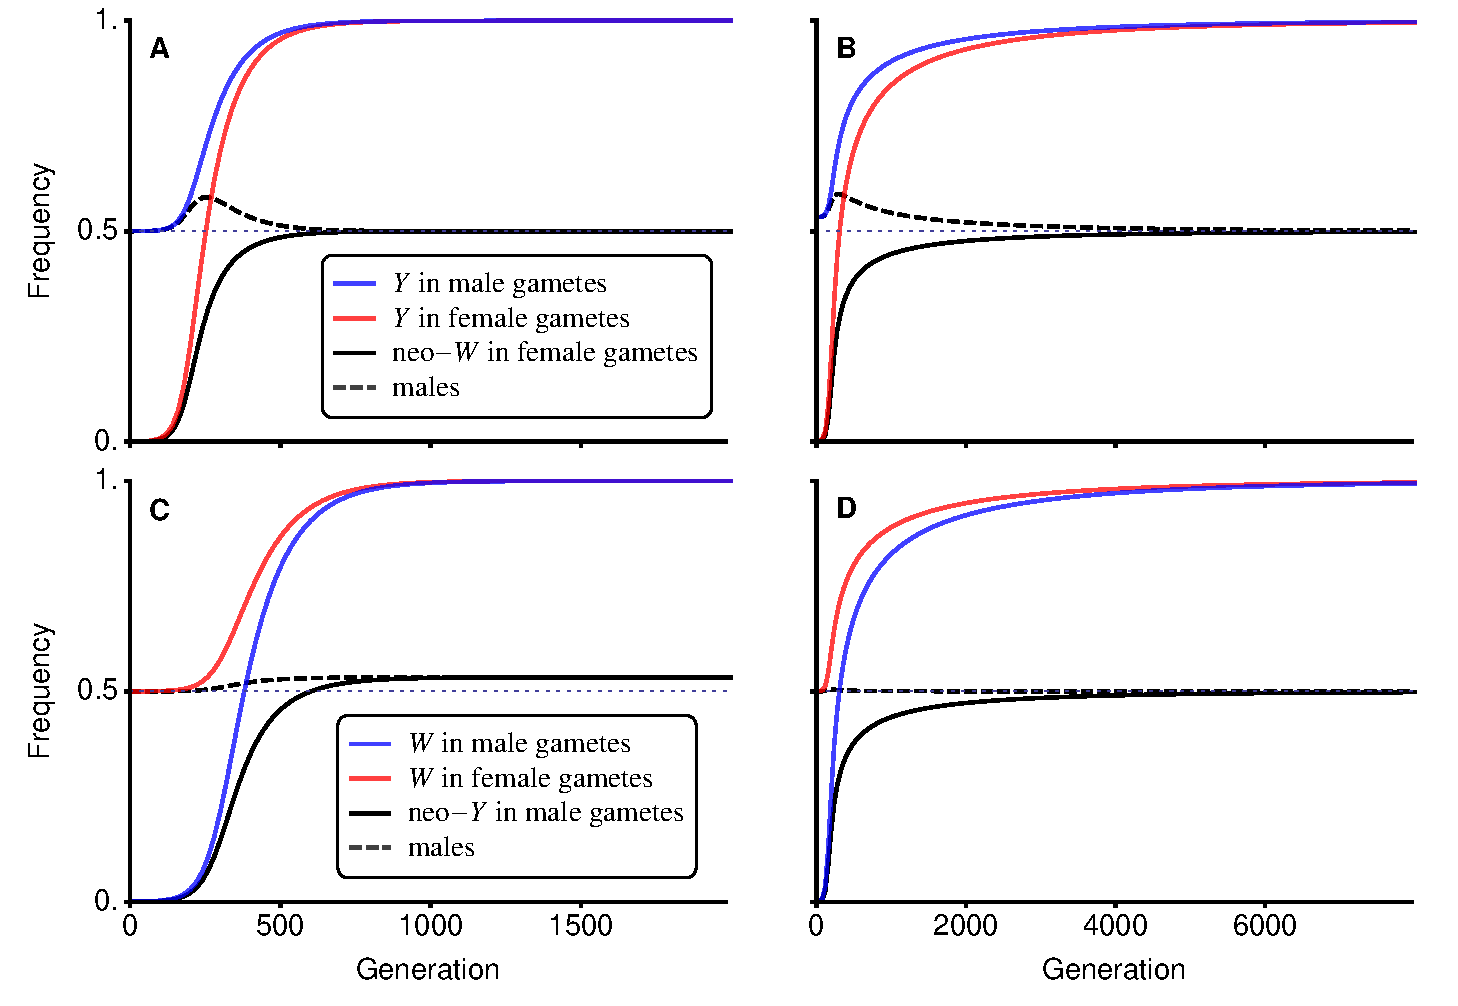
\includegraphics[width=\linewidth]{Combination_Turnover}\\
\caption{
Heterogametic transitions from XY to ZW sex determination (neo-W frequency shown by black lines, panels A and B) or from ZW to XY (neo-Y frequency shown by black lines, panels C and D) occur similarly regardless of sex ratio biases present before (B versus D) or after (C versus A, dashed lines show male frequency). 
During invasion by a neo-ZW sex determination system (A and B), the ancestral Y fixes in both males and females (blue and red lines). 
Similarly, the ancestral W allele fixes in males and females (blue and red lines) during a ZW to XY transition. 
In this plot, there is no gametic competition ($t^\female=t^\male=0$) and meiotic drive occurs during male meiosis only ($\alpha^\female_{\Delta}=0$, $\alpha^\male_{\Delta}=-1/5$). Therefore, sex ratio biases can only arise when the \textbf{A} locus is linked to an XY sex-determining locus.
In panels A and C, the neo-sex-determining locus is more closely linked to the \textbf{A} locus than the ancestral sex-detemining region ($r=1/2$, $R=1/20$) such that a neo-Y can caused biased sex ratios (panel C).
In panels B and D, the ancestral sex-determining locus is more closely linked to the \textbf{A} locus than the neo-sex-detemining locus ($r=1/20$, $R=1/2$). 
Therefore, an ancestral XY sex determination can have a biased zygotic sex ratio that becomes unbiased after an unlinked neo-W invades (B). 
However, in panel D, a unlinked neo-Y invades an ancestral ZW sex determination system in a similar manner but no biases to the zygotic sex ratio occur. 
With diploid selection alone, neo-sex-determining loci do not spread if they are less closely linked to the \textbf{A} locus than the ancestral sex-determining locus (see equation \eqref{eq:lambda_neoW} and Figure \ref{fig:Combination_Centimorgans}A). 
In this plot there are no sex differences in selection and an equilibrium is maintained because selection in diploids opposes meiotic drive, $s^\female =s^\male = 1/5$, $h^\female = h^\male = 7/10$.
\textcolor{red}{Aesthetic adjustments: Could add titles to the columns/rows: neo-W for row 1, neo-Y for row 3, $r=0.5$, $R=0.05$ for column 1 and $r=0.05$, $R=0.5$ for column 2. Could adjust padding (too much whitespace where there is no axis label). It also seems could increase ratio of font size relative to plot size to make figure more compact. Matt - could you uncomment the line legends in the Mathematica file (function not included in my Mathematica version).}
}
\label{fig:Combination_Turnover}
\end{figure}
%%%%%%%%%%%%%%%%%%%%%%%%%%%%%%%%%%%%%%%%%%%%%%%%%%%%%%%%%
\newpage

%%%%%%%%%%%%%%%%%%%%%%%%%%%%%%%%%%%%%%%%%%%%%%%%%%%%%%%%%
%Changes in mean fitness
%%%%%%%%%%%%%%%%%%%%%%%%%%%%%%%%%%%%%%%%%%%%%%%%%%%%%%%%%
\begin{figure}[!h]
\centering
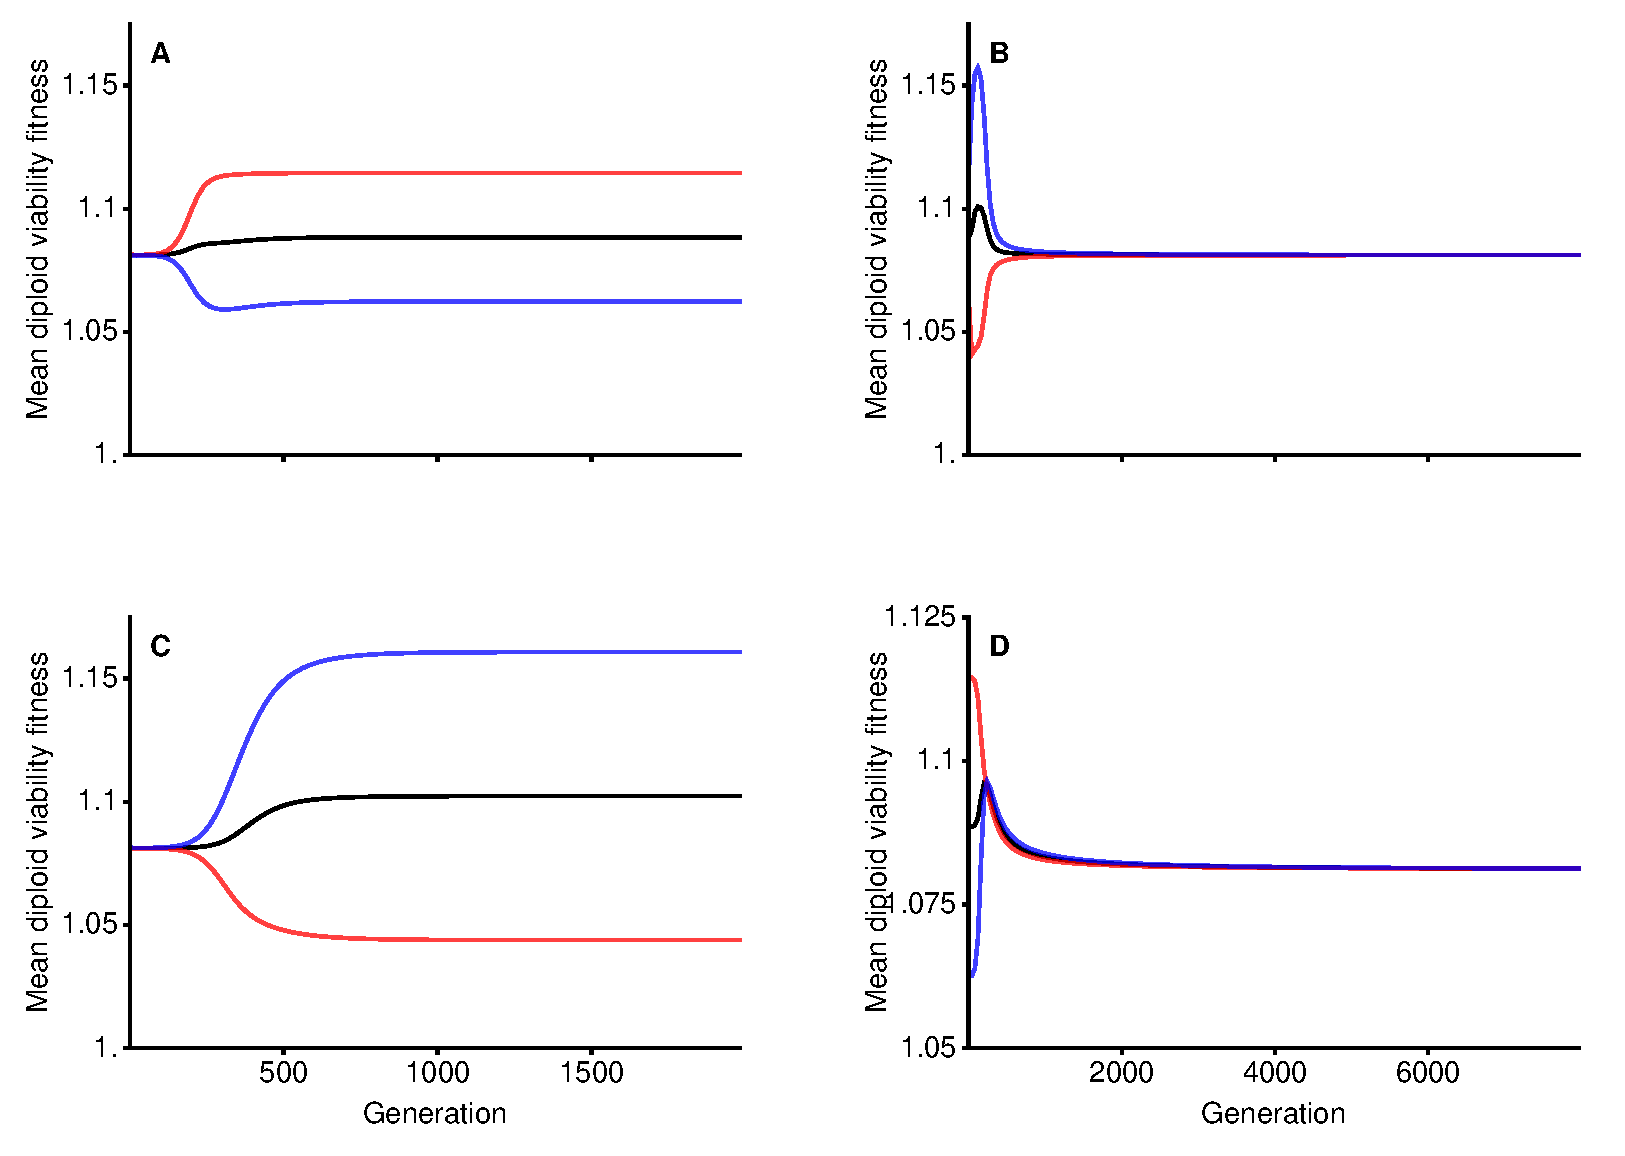
\includegraphics[width=\linewidth]{Combination_MeanFit}\\
\caption{
Here, we plot how male mean fitness (blue lines), female mean fitness (red lines), and population mean fitness (male mean fitness plus female mean fitness, black lines) changes during the transitions between sex-determination systems shown in Figure \ref{fig:Combination_Turnover}. 
Here we multiply male mean fitness and female mean fitness by two so that we can show it on the same scale as population mean fitness. 
The mean fitness of females increases during the spread of neo-W alleles (A and B) and the mean fitness of males increases during the spread of neo-Y alleles (C and D). 
However, when a neo-sex determining system evolves that is less closely linked to a locus under selection (B and D), population mean fitness decreases. 
\textcolor{red}{
Could add titles to the columns/rows: neo-W for row 1, neo-Y for row 3, $r=0.5$, $R=0.05$ for column 1 and $r=0.05$, $R=0.5$ for column 2. \& possibly adjust padding (too much whitespace?). Matt - could you uncomment the line legends in the Mathematica file (function not included in my Mathematica version).}
}
\label{fig:Combination_MeanFit}
\end{figure}
%%%%%%%%%%%%%%%%%%%%%%%%%%%%%%%%%%%%%%%%%%%%%%%%%%%%%%%%%
\newpage

%%%%%%%%%%%%%%%%%%%%%%%%%%%%%%%%%%%%%%%%%%%%%%%%%%%%%%%%%
%Chromosomal Positions
%%%%%%%%%%%%%%%%%%%%%%%%%%%%%%%%%%%%%%%%%%%%%%%%%%%%%%%%%
\begin{figure}[!h]
\centering
%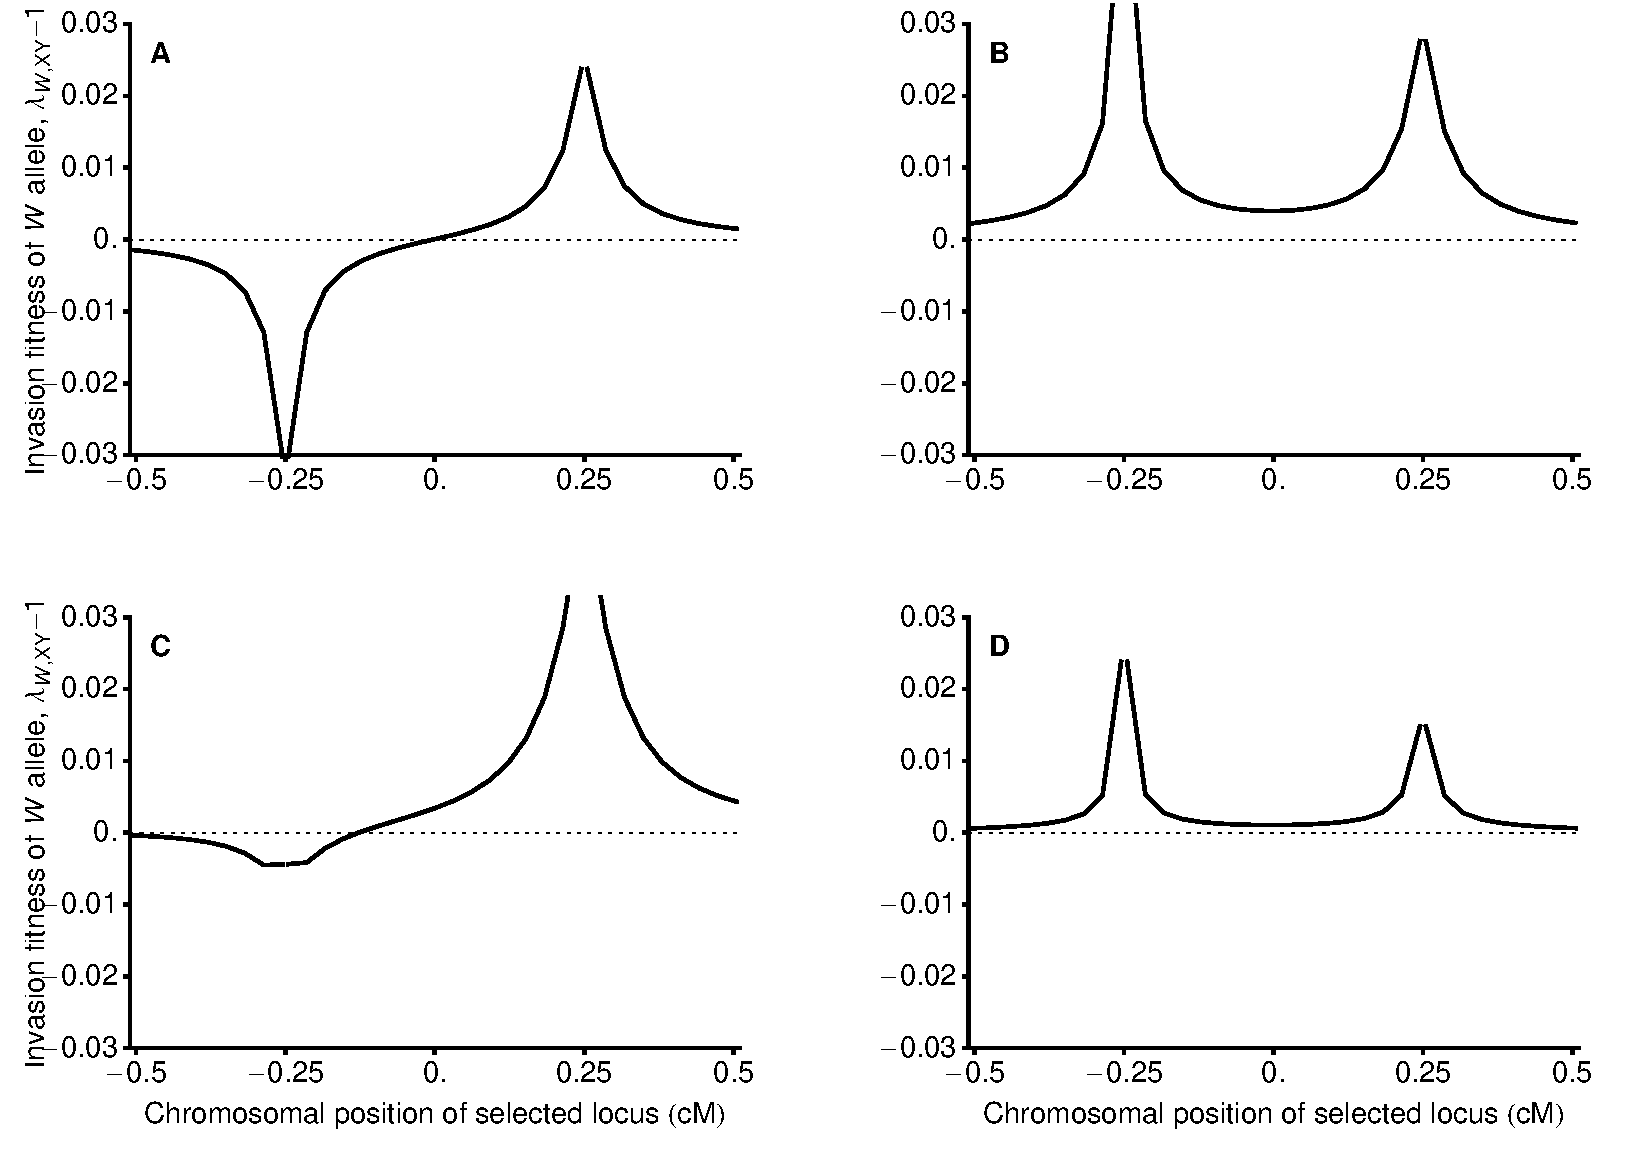
\includegraphics[width=\linewidth]{Combination_Centimorgan}\\
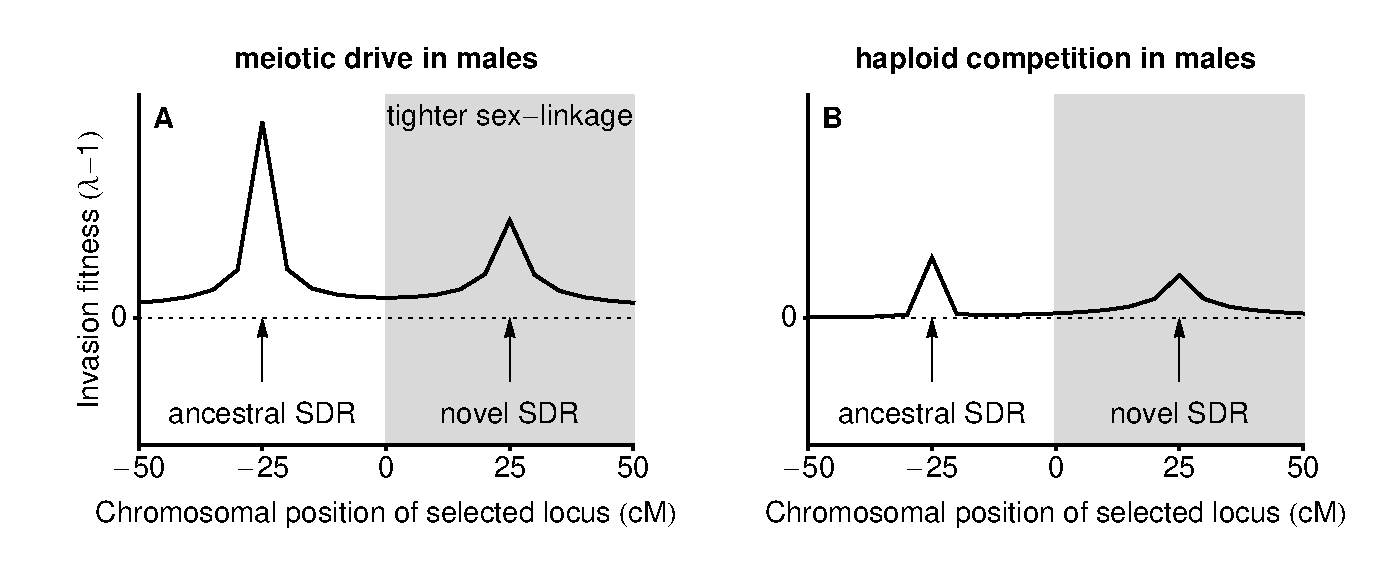
\includegraphics[width=\linewidth]{PositionPlot}\\
\caption{
The invasion fitness of a neo-W allele plotted against the relative location of a locus under direct selection, \textbf{A}, for various selective regimes. 
We assume that the ancestral sex-determining locus is located at -0.25, the novel sex-determining locus is located at 0.25 and that there is a polymorphism at the \textbf{A} locus maintained by selection.
We used Haldane's map function \citep[Equation 3 in ][]{Haldane1919} to convert from map distance (centiMorgans) to the probability of a cross-over event. 
In A, there is no haploid selection ($t^\Hermaphrodite=\alpha^\Hermaphrodite_{\Delta}=0$) and selection in diploids is sexually antagonistic \citep[following][]{vanDoorn:2010hu}, in which case a neo-W can only invade if it is more closely linked to the selected locus ($s^\female=1/10$, $h^\female=7/10$ $s^\male=-1/10$, $h^\male=3/10$).
In B-D we include haploid selection and assume that selection in diploids is not sexually-antagonistic ($s^\female s^\male>0$). 
A polymorphism can then be maintained by opposing selection between the haploid and diploid phases. 
In B, there is drive in favour of the $a$ allele in males ($\alpha^\male_{\Delta}=-1/10$), no female meiotic drive or gametic competition, $t^\Hermaphrodite=\alpha^\female_{\Delta}=0$), and equal selection in diploid sexes ($s^\female=s^\male=1/10$, $h^\female=h^\male=7/10$). In this case, a neo-W can invade even when the selected locus is more closely linked to the ancestral sex determining locus (see Table \ref{tab:specialcases} and Figure \ref{fig:Combination_Turnover}). 
In C and D, there is gametic competition among male gametes only (favouring $a$, $t^\male=-1/10$) and no meiotic drive or gametic competition in females ($t^\female=\alpha^\Hermaphrodite_{\Delta}=0$). 
In this case, the neo-W does not invade if $s^\female>s^\male$ (panel C: $s^\female=3/20$, $s^\male=1/20$) but does if $s^\female<s^\male$ (panel D: $s^\female=1/20$, $s^\male=3/20$), see Table \ref{tab:specialcases}.
\textcolor{red}{I suspect that panel C has a region where no equilibrium is maintained (CHECK! Maybe include different parameters here or remove the part when no equilibrium). Currently use different parameters for B than using in figure \ref{fig:Combination_Turnover} (selection/drive twice as strong in turnover figure). This plot would also benefit from titles giving, e.g., ``sexually-antagonistic selection, $s^\female s^\male<0$'' for A, ``male meiotic drive, $s^\female s^\male>0$'' for B}
}
\label{fig:Combination_Centimorgans}
\end{figure}
%%%%%%%%%%%%%%%%%%%%%%%%%%%%%%%%%%%%%%%%%%%%%%%%%%%%%%%%%
\newpage


%%%%%%%%%%%%%%%%%%%%%%%%%%%%%%%%%%%%%%%%%%%%%%%%%%%%%%%%%
%W invades XY and fixes
%%%%%%%%%%%%%%%%%%%%%%%%%%%%%%%%%%%%%%%%%%%%%%%%%%%%%%%%%
%\begin{figure}
%\centering
%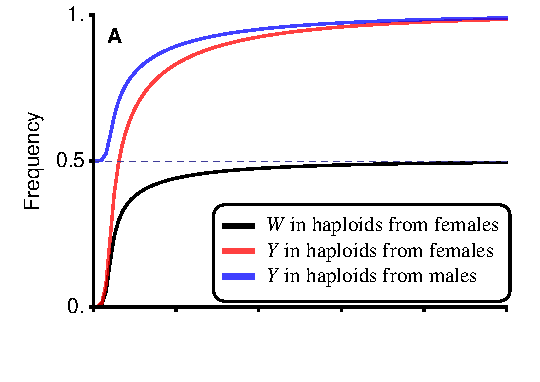
\includegraphics[width=0.5\linewidth]{FreqWLowR}\\
%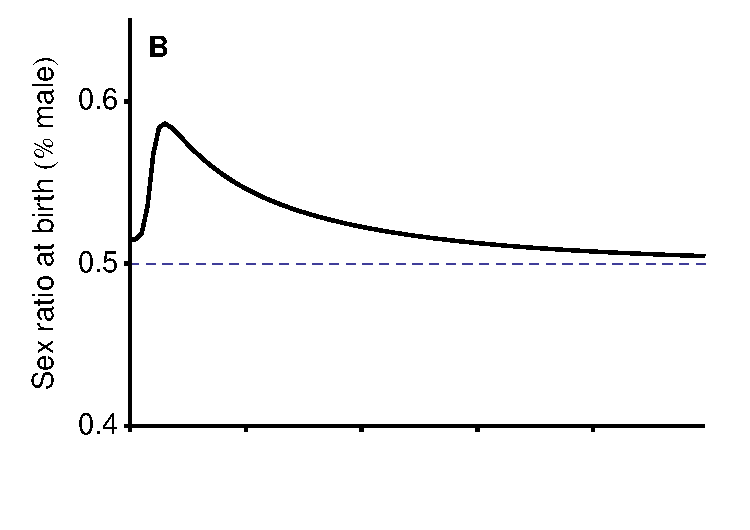
\includegraphics[width=0.5\linewidth]{SexRatioLowR}\\
%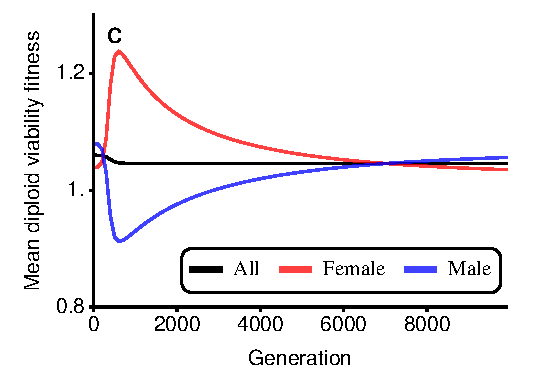
\includegraphics[width=0.5\linewidth]{MeanDipFitLowR}
%\caption{
%Haploid selection allows a neo-$W$ to invade an ancestral $XY$ system and fix (\textbf{A}) despite temporarily biasing the sex ratio further (\textbf{B}) and decreasing mean diploid viability fitness (\textbf{C}).
%Complete turnover between genetic sex-determination systems occurs despite the neo-$W$ being less tightly linked to the selected locus than the ancestral sex-determining locus is, $R>r$.
%Parameters: $k=1$, $s^\female = 0.05$, $s^\male = 0.15$, $h^\female = h^\male = 0.7$, $t^\female = 0$, $t^\male = -0.1$, $\alpha^\male = \alpha^\female = 1/2$, $r=0.01$, $R=0.05$.
%}
%\label{fig:WinvasionLowR}
%\end{figure}
%%%%%%%%%%%%%%%%%%%%%%%%%%%%%%%%%%%%%%%%%%%%%%%%%%%%%%%%%

%%%%%%%%%%%%%%%%%%%%%%%%%%%%%%%%%%%%%%%%%%%%%%%%%%%%%%%%%
%W invades XY but does not fix
%%%%%%%%%%%%%%%%%%%%%%%%%%%%%%%%%%%%%%%%%%%%%%%%%%%%%%%%%
%\begin{figure}
%\centering
%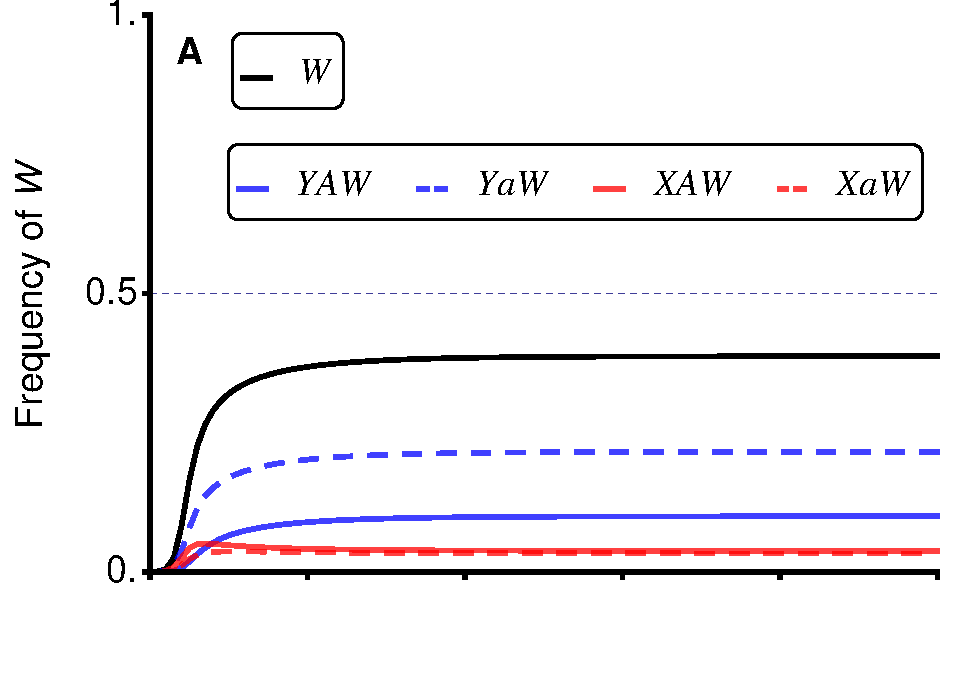
\includegraphics[width=0.5\linewidth]{FreqWHighR}\\
%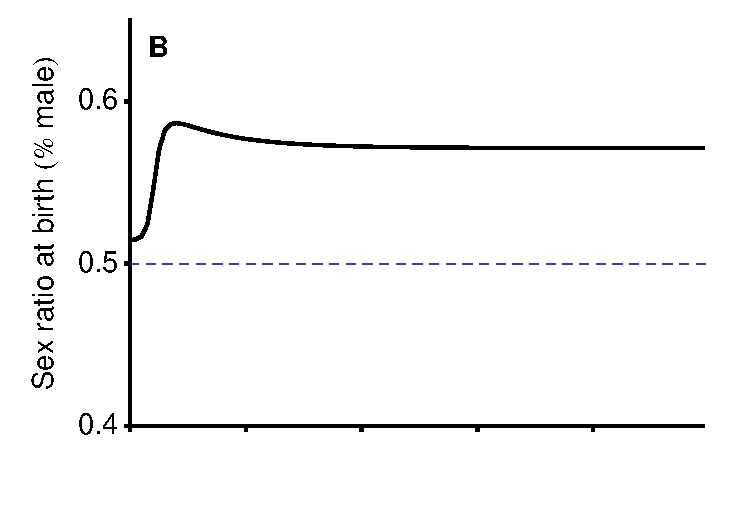
\includegraphics[width=0.5\linewidth]{SexRatioHighR}\\
%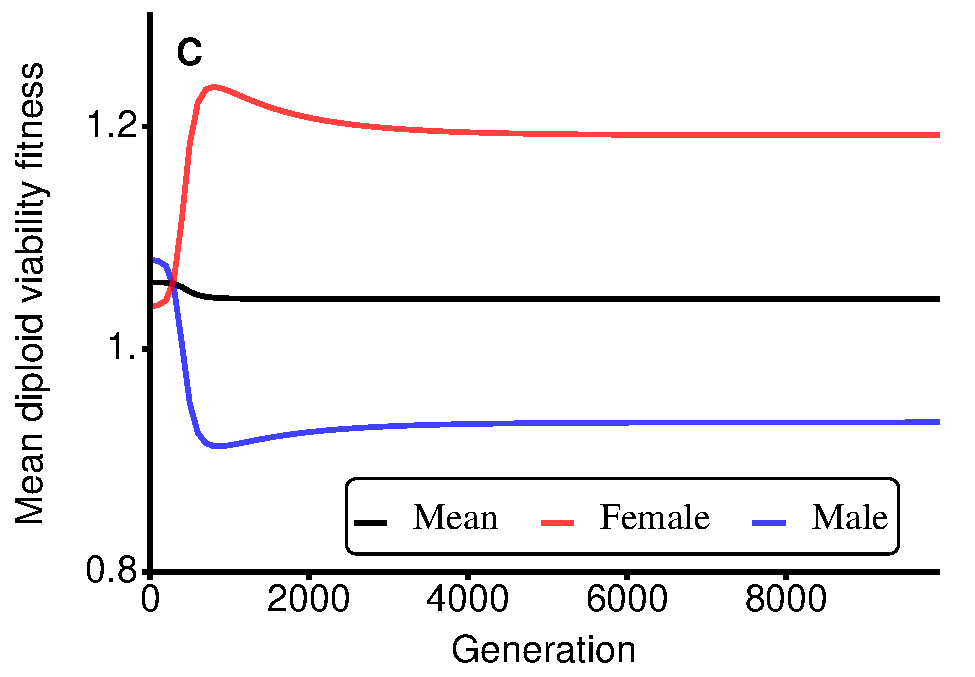
\includegraphics[width=0.5\linewidth]{MeanDipFitHighR}
%\caption{
%Haploid selection allows a completely unlinked neo-$W$ to invade an ancestral $XY$ system (\textbf{A}) despite further biasing the sex ratio (\textbf{B}) and decreasing mean diploid viability fitness (\textbf{C}).
%The neo-$W$ does not fix (although variation at the \textbf{A} locus is maintained, $V_A>0$), resulting in a polymorphic sex-determination system.
%Parameters as in Figure \ref{fig:WinvasionLowR} but with $R=0.5$.
%}
%\label{fig:WinvasionHighR}
%\end{figure}
%%%%%%%%%%%%%%%%%%%%%%%%%%%%%%%%%%%%%%%%%%%%%%%%%%%%%%%%%

%%%%%%%%%%%%%%%%%%%%%%%%%%%%%%%%%%%%%%%%%%%%%%%%%%%%%%%%%
%W invades for all rates of recombination with selected locus
%%%%%%%%%%%%%%%%%%%%%%%%%%%%%%%%%%%%%%%%%%%%%%%%%%%%%%%%%
%\begin{figure}
%\centering
%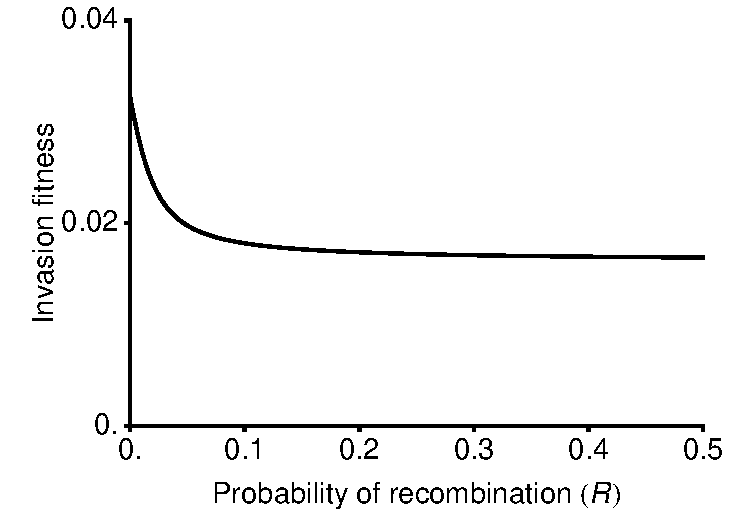
\includegraphics[width=0.5\linewidth]{InvasionVsRecombination}
%\caption{
%A neo-$W$ invades an ancestral $XY$ system with haploid selection regardless of how tightly it is linked to the selected locus. 
%Parameters as in Figure \ref{fig:WinvasionLowR}.
%}
%\label{fig:InvasionVsRecombination}
%\end{figure}
%%%%%%%%%%%%%%%%%%%%%%%%%%%%%%%%%%%%%%%%%%%%%%%%%%%%%%%%%

%%%%%%%%%%%%%%%%%%%%%%%%%%%%%%%%%%%%%%%%%%%%%%%%%%%%%%%%%
%W invasion versus position of selected locus
%%%%%%%%%%%%%%%%%%%%%%%%%%%%%%%%%%%%%%%%%%%%%%%%%%%%%%%%%
%\begin{figure}
%\centering
%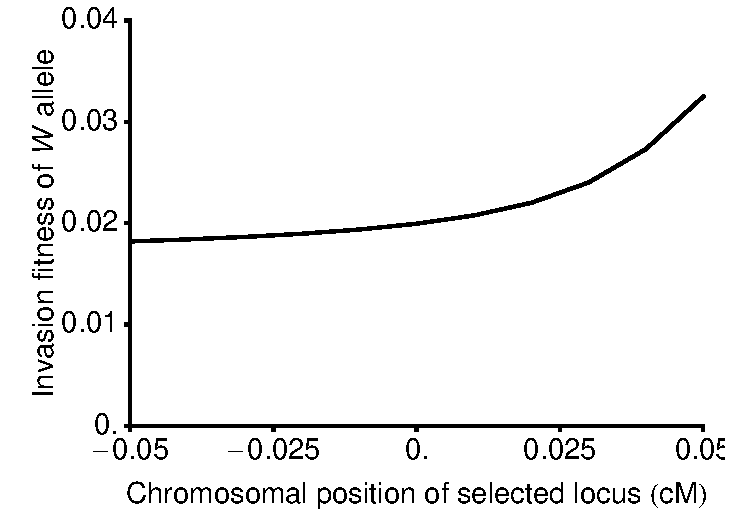
\includegraphics[width=0.5\linewidth]{InvasionVsCentiMorgans}
%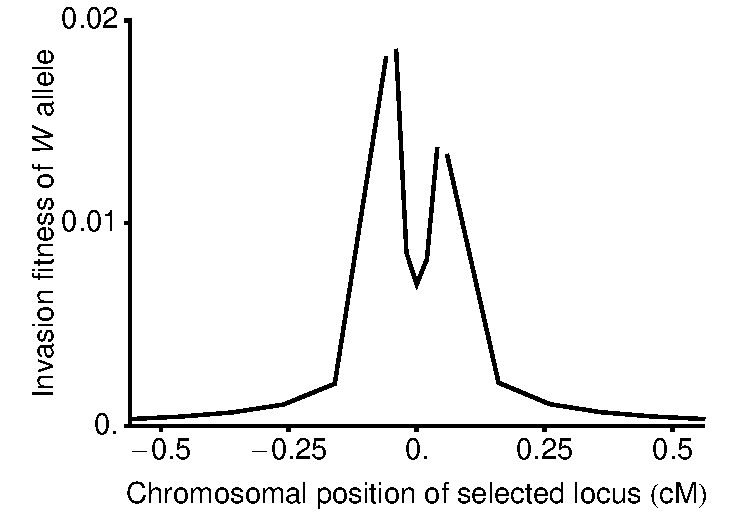
\includegraphics[width=0.5\linewidth]{InvasionVsCentiMorgansAllOrders}
%\caption{
%Haploid selection allows a neo-$W$ to invade an ancestral $XY$ system regardless of how tightly it and the ancestral sex-determining locus are linked to the selected locus. 
%The ancestral sex-determining locus is located at -0.05 and the novel sex-determining locus is located at 0.05 (corresponding to the peaks of invasion fitness), such that the probability of a cross-over between them is $\approx0.1$.
%The x-axis gives the position of the locus under haploid selection.
%We used Haldane's map function \citep[Equation 3 in ][]{Haldane1919} to convert from map distance (centiMorgans) to the probability of a cross-over event. 
%Parameters as in Figure \ref{fig:WinvasionLowR}.
%}
%\label{fig:InvasionVsCentiMorgans}
%\end{figure}
%%%%%%%%%%%%%%%%%%%%%%%%%%%%%%%%%%%%%%%%%%%%%%%%%%%%%%%%%

%%%%%%%%%%%%%%%%%%%%%%%%%%%%%%%%%%%%%%%%%%%%%%%%%%%%%%%%%
%Y invades ZW and fixes (counter example to Kozi explanation)
%%%%%%%%%%%%%%%%%%%%%%%%%%%%%%%%%%%%%%%%%%%%%%%%%%%%%%%%%
%\begin{figure}
%\centering
%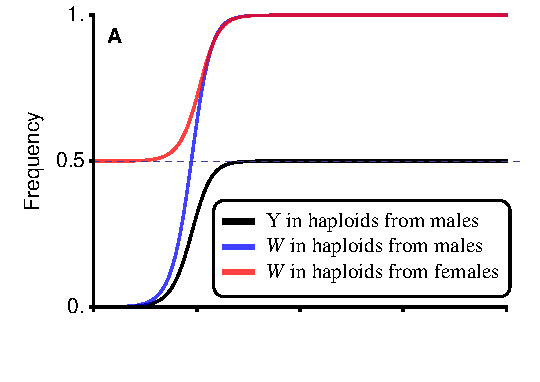
\includegraphics[width=0.5\linewidth]{FreqWCounterKozi}\\
%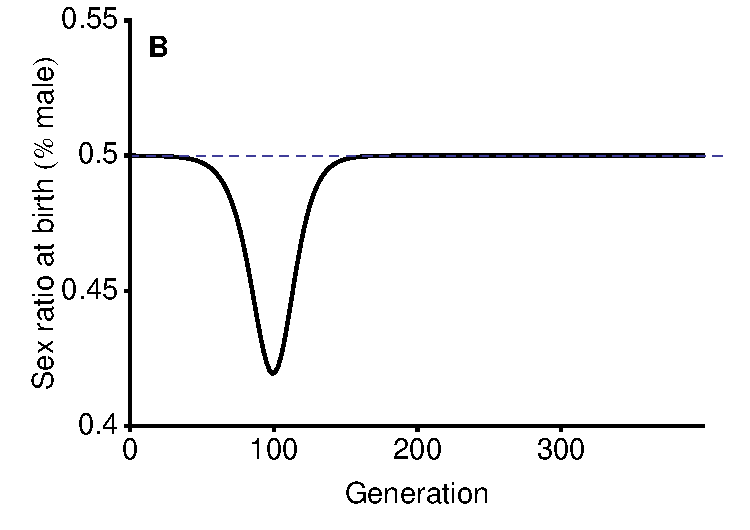
\includegraphics[width=0.5\linewidth]{SexRatioCounterKozi}\\
%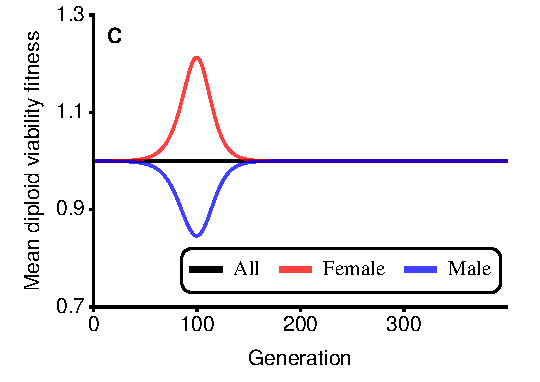
\includegraphics[width=0.5\linewidth]{MeanDipFitCounterKozi}
%\caption{
%Meiotic drive allows a neo-$Y$ to invade an ancestral $ZW$ system and fix (\textbf{A}) despite temporarily biasing the sex ratio (\textbf{B}). %and decreasing mean diploid viability fitness (\textbf{C}).
%Parameters: $k=0$, $s^\female = s^\male = t^\female = t^\male = 0$, $\alpha^\male = 0.4$, $\alpha^\female = 1/2$, $r=0$, $R=0$.
%}
%\label{fig:CounterKozi}
%\end{figure}
%%%%%%%%%%%%%%%%%%%%%%%%%%%%%%%%%%%%%%%%%%%%%%%%%%%%%%%%%

\setcounter{equation}{0}
\renewcommand{\theequation}{S.\arabic{equation}}
\setcounter{figure}{0}
\renewcommand{\thefigure}{S.\arabic{figure}}
\setcounter{table}{0}
\renewcommand{\thetable}{S.\arabic{table}}

%%%%%%%%%%%%%%%%%%%%%%%%%%%%%%%%%%%%%%%%%%%%%%%%%%%%%%%%%
\newpage

\section*{Appendix}

\subsection*{Recursion Equations}
\label{app:recurs}

In each generation we census the genotype frequencies in male and female gametes/gametophytes (hereafter, gametes) after meiosis (and any meiotic drive) and immediately before gametic competition. 
At this stage, the frequencies of X-bearing male and female gametes are given by $X_{i}^{\male}$ and $X_{i}^{\female}$ and the frequencies of Y-bearing gametes are given by $Y_{i}^{\male}$ and $Y_{i}^{\female}$ where the index $i$ specifies genotypes $MA=1$, $Ma=2$, $mA=3$, and $ma=4$ ($\sum_{i=1}^{4}Y_{i}^{\male}+X_{i}^{\male}=1$ and $\sum_{i=1}^{4}Y_{i}^{\female}+X_{i}^{\female}=1$). 
Competition then occurs among gametes of the same sex (e.g., among eggs and among sperm separately) according to the \textbf{A} locus allele, $g$ ($g\in A$, $a$, see Table \ref{tab:fitnesstable}), carried by individuals with genotype $i$.
The genotype frequencies after gametic competition are $X_{i}^{\Hermaphrodite,s}= w_{g}X_{i}^{\Hermaphrodite}/\bar{w}_{H}^{\Hermaphrodite}$ and $Y_{i}^{\Hermaphrodite,s}= w_{g}Y_{i}^{\Hermaphrodite}/\bar{w}_{H}^{\Hermaphrodite}$, where $\bar{w}_{H}^{\Hermaphrodite}=\sum_{i=1}^{4} w_{g}X_{i}^{\Hermaphrodite}+w_{g}Y_{i}^{\Hermaphrodite}$ is the mean fitness of male ($\Hermaphrodite=\male$) or female ($\Hermaphrodite=\female$) gametes. 
Random mating then occurs between gametes to produce diploid zygotes with genotype $ij$ at the \textbf{A} and \textbf{M} loci, such that $XX$ zygotes are denoted $xx_{ij}$, $XY$ zygotes are $xy_{ij}$, and $YY$ zygotes are $yy_{ij}$. 
In $XX$ and $YY$ zygotes, individuals with genotype $ij$ are equivalent to those with genotype $ji$; for simplicity, we denote the frequency of genotype $ij$ to the average of these frequencies, $xx_{ij}=(X_{i}^{\female,s}X_{j}^{\male,s}+X_{j}^{\female,s}X_{i}^{\male,s})/2$ and $yy_{ij}=(Y_{i}^{\female,s}Y_{j}^{\male,s}+Y_{j}^{\female,s}Y_{i}^{\male,s})/2$. 

Denoting the \textbf{M} locus genotype by $b$ ($b\in MM$, $Mm$, $mm$) and the \textbf{X} locus genotype by $c$ ($c\in XX$, $XY$, $YY$), zygotes develop as females with probability $k_{bc}$. 
Therefore, the frequencies of $XX$ females are given by $xx_{ij}^{\female}=k_{bc}xx_{ij}$, $XY$ females are given by $xy_{ij}^{\female}=k_{bc}xy_{ij}$, and $YY$ females are given by $yy_{ij}^{\female}=k_{bc}xy_{ij}$. 
Similarly, $XX$ male frequencies are $xx_{ij}^{\male}=(1-k_{bc})xx_{ij}$, $XY$ male frequencies are $xy_{ij}^{\male}=(1-k_{bc})xy_{ij}$, and $YY$ males frequencies are $yy_{ij}^{\male}=(1-k_{bc})xy_{ij}$.
This notation allows both the ancestral and novel sex-determining regions to determine zygotic sex according to an $XY$ system, a $ZW$ system, or an environmental sex-determining system. 
In addition, we can consider any epistatic dominance relationship between the two sex-determining loci. 
Typically, we assume that the ancestral sex-determining system (\textbf{X} locus) is $XY$ ($k_{MMXX}=1$ and $k_{MMXY}=k_{MMYY}=0$) and epistatically recessive to a dominant novel sex-determining locus, \textbf{M} ($k_{Mmc}=k_{mmc}=k$). 


Selection among diploids then occurs according to the diploid genotype at the \textbf{A} locus, $h$, for an individual of type $ij$ ($h \in AA$, $Aa$, $aa$, see Table \ref{tab:fitnesstable}). 
The diploid frequencies after selection in sex $\Hermaphrodite$ are given by $xx_{ij}^{\Hermaphrodite,s}=w_{h}^{\Hermaphrodite} xx_{ij}/\bar{w}^{\Hermaphrodite}$, $xy_{ij}^{\Hermaphrodite,s}=w_{h}^{\Hermaphrodite} xy_{ij}/\bar{w}^{\Hermaphrodite}$, and $yy_{ij}^{\Hermaphrodite,s}=w_{h}^{\Hermaphrodite} yy_{ij}/\bar{w}^{\Hermaphrodite}$, where $\bar{w}^{\Hermaphrodite}= \sum_{i=1}^{4}\sum_{j=1}^{4}w_{h}^{\Hermaphrodite}xx_{ij}+w_{h}^{\Hermaphrodite}xy_{ij}+w_{h}^{\Hermaphrodite}yy_{ij}$ is the mean fitness of individuals of sex $\Hermaphrodite$. 

Finally, these diploids undergo meiosis to produce the next generation of gametes. 
Recombination and sex-specific meiotic drive occur during meiosis.
%We can also assume that recombination is sex specific and/or affected by the M locus - but generally we don't so I just describe $R=R_{f}=R, r_{MM,d}=r_{Mm,d}=r_{mm,d}=r, \chi_{m}=\chi_{f}=\chi$.
Here, we allow the relative locations of the SDR, \textbf{A}, and \textbf{M} loci to be generic by using three parameters to describe the recombination rates between them. $R$ is the recombination rate between the \textbf{A} locus and the \textbf{M} locus, $\chi$ is the recombination rate between the \textbf{M} locus and the \textbf{X} locus, and $r$ is the recombination rate between the \textbf{A} locus and the \textbf{X} locus. 
Table \ref{tab:chisubstitutions} gives substitutions for $\chi$ for defined relative locations of these loci.
During meiosis in sex $\Hermaphrodite$, meiotic drive occurs such that, in $Aa$ heterozygotes, a fraction $\alpha^{\Hermaphrodite}$ of gametes produced carry the $A$ allele and $(1-\alpha^\Hermaphrodite)$ carry the $a$ allele. 

\begin{table}[ht]
\centering
\smallskip
\caption{$\chi$ substitutions for different loci orders (assuming no interference)}
\begin{tabular}{l l}
\hline\hline
  Order of loci &   \\ [0.5ex] \hline
  SDR-A-M & $\chi=R(1-r)+r(1-R)$  \\
  SDR-M-A & $\chi=(r-R)/(1-2R)$ \\
  A-SDR-M & $\chi=(R-r)/(1-2r)$ \\
  \hline \hline
  \label{tab:chisubstitutions}
 \end{tabular}
\end{table}

Among gametes from sex $\Hermaphrodite$ (sperm/pollen when $\Hermaphrodite=\male$, eggs/ovules when $\Hermaphrodite=\female$), the frequencies of haplotypes (before gametic competition) in the next generation are given by

\begingroup
\allowdisplaybreaks
\begin{subequations}
\begin{align}
%
\begin{split}
X_{MA}^{{\Hermaphrodite}'}=&xx_{11}^{\Hermaphrodite,s}+xx_{13}^{\Hermaphrodite,s}/2+(xx_{12}^{\Hermaphrodite,s}+xx_{14}^{\Hermaphrodite,s})\alpha^\Hermaphrodite\\
&-R(xx_{14}^{\Hermaphrodite,s}-xx_{23}^{\Hermaphrodite,s}) \alpha^\Hermaphrodite\\
&+(xy_{11}^{\Hermaphrodite,s}+xy_{13}^{\Hermaphrodite,s})/2+(xy_{12}^{\Hermaphrodite,s}+xy_{14}^{\Hermaphrodite,s})\alpha^\Hermaphrodite\\
&- r(xy_{12}^{\Hermaphrodite,s}-xy_{21}^{\Hermaphrodite,s})\alpha^\Hermaphrodite - \chi(xy_{13}^{\Hermaphrodite,s}-xy_{31}^{\Hermaphrodite,s})/2\\
&+\big{\{}-(R+r+\chi)xy_{14}^{\Hermaphrodite,s} +(r+\chi-R)xy_{41}^{\Hermaphrodite,s}\\
&+(R+r-\chi) xy_{23}^{\Hermaphrodite,s}+(R+\chi-r)xy_{32}^{\Hermaphrodite,s}\big{\}}\alpha^\Hermaphrodite/2
\end{split}
\\
%
\begin{split}
X_{Ma}^{{\Hermaphrodite}'}=&xx_{22}^{\Hermaphrodite,s}+xx_{24}^{\Hermaphrodite,s}/2+(xx_{12}^{\Hermaphrodite,s}+xx_{23}^{\Hermaphrodite,s})\alpha^\Hermaphrodite\\
&-R(xx_{23}^{\Hermaphrodite,s}-xx_{14}^{\Hermaphrodite,s}) \alpha^\Hermaphrodite\\
&(xy_{22}^{\Hermaphrodite,s}+xy_{24}^{\Hermaphrodite,s})/2+(xy_{21}^{\Hermaphrodite,s}+xy_{23}^{\Hermaphrodite,s})(1-\alpha^\Hermaphrodite)\\
&- r(xy_{21}^{\Hermaphrodite,s}-xy_{12}^{\Hermaphrodite,s})(1-\alpha^\Hermaphrodite) - \chi(xy_{24}^{\Hermaphrodite,s}-xy_{42}^{\Hermaphrodite,s})/2\\
&+\big{\{}-(R+r+\chi)xy_{23}^{\Hermaphrodite,s}+(r+\chi-R)xy_{32}^{\Hermaphrodite,s}\\
&+(R+r-\chi) xy_{14}^{\Hermaphrodite,s}+(R+\chi-r)xy_{41}^{\Hermaphrodite,s}\big{\}}(1-\alpha^\Hermaphrodite)/2
\end{split}
\\
%
\begin{split}
X_{mA}^{{\Hermaphrodite}'}=&xx_{33}^{\Hermaphrodite,s}+xx_{13}^{\Hermaphrodite,s}/2+(xx_{23}^{\Hermaphrodite,s}+xx_{34}^{\Hermaphrodite,s})\alpha^\Hermaphrodite\\
&-R(xx_{23}^{\Hermaphrodite,s}-xx_{14}^{\Hermaphrodite,s}) \alpha^\Hermaphrodite\\
&(xy_{33}^{\Hermaphrodite,s}+xy_{31}^{\Hermaphrodite,s})/2+(xy_{32}^{\Hermaphrodite,s}+xy_{34}^{\Hermaphrodite,s})\alpha^\Hermaphrodite\\
&- r(xy_{34}^{\Hermaphrodite,s}-xy_{43}^{\Hermaphrodite,s}) \alpha^\Hermaphrodite - \chi(xy_{31}^{\Hermaphrodite,s}-xy_{13}^{\Hermaphrodite,s})/2\\
&+\big{\{}-(R+r+\chi)xy_{32}^{\Hermaphrodite,s} +(r+\chi-R)xy_{23}^{\Hermaphrodite,s}\\
&+(R+r-\chi) xy_{41}^{\Hermaphrodite,s}+(R+\chi-r)xy_{14}^{\Hermaphrodite,s}\big{\}} \alpha^\Hermaphrodite/2
\end{split}
\\
%
\begin{split}
X_{ma}^{{\Hermaphrodite}'}=&xx_{44}^{\Hermaphrodite,s}+xx_{34}^{\Hermaphrodite,s}/2+(xx_{14}^{\Hermaphrodite,s}+xx_{24}^{\Hermaphrodite,s})\alpha^\Hermaphrodite\\
&-R(xx_{14}^{\Hermaphrodite,s}-xx_{23}^{\Hermaphrodite,s}) \alpha^\Hermaphrodite\\
&(xy_{44}^{\Hermaphrodite,s}+xy_{42}^{\Hermaphrodite,s})/2+(xy_{41}^{\Hermaphrodite,s}+xy_{43}^{\Hermaphrodite,s})(1-\alpha^\Hermaphrodite)\\
&- r(xy_{43}^{\Hermaphrodite,s}-xy_{34}^{\Hermaphrodite,s})(1-\alpha^\Hermaphrodite) - \chi(xy_{42}^{\Hermaphrodite,s}-xy_{24}^{\Hermaphrodite,s})/2\\
&+\big{\{}-(R+r+\chi)xy_{41}^{\Hermaphrodite,s}+(r+\chi-R)xy_{14}^{\Hermaphrodite,s}\\
&+(R+r-\chi) xy_{32}^{\Hermaphrodite,s}+(R+\chi-r)xy_{23}^{\Hermaphrodite,s}\big{\}}(1-\alpha^\Hermaphrodite)/2
\end{split}
\\
\begin{split}
Y_{MA}^{{\Hermaphrodite}'}=&yy_{11}^{\Hermaphrodite,s}+yy_{13}^{\Hermaphrodite,s}/2+(yy_{12}^{\Hermaphrodite,s}+yy_{14}^{\Hermaphrodite,s})\alpha^\Hermaphrodite\\
&-R(yy_{14}^{\Hermaphrodite,s}-yy_{23}^{\Hermaphrodite,s}) \alpha^\Hermaphrodite\\
&(xy_{11}^{\Hermaphrodite,s}+xy_{31}^{\Hermaphrodite,s})/2+(xy_{21}^{\Hermaphrodite,s}+xy_{41}^{\Hermaphrodite,s})\alpha^\Hermaphrodite\\
&- r(xy_{21}^{\Hermaphrodite,s}-xy_{12}^{\Hermaphrodite,s})\alpha^\Hermaphrodite - \chi(xy_{31}^{\Hermaphrodite,s}-xy_{13}^{\Hermaphrodite,s})/2\\
&+\big{\{} - (R+r+\chi)xy_{41}^{\Hermaphrodite,s} + (r+\chi-R)xy_{14}^{\Hermaphrodite,s}\\
& + (R+r-\chi)xy_{32}^{\Hermaphrodite,s} + (R+\chi-r) xy_{23}^{\Hermaphrodite,s}\big{\}}\alpha^\Hermaphrodite/2
\end{split}
\\
%
\begin{split}
Y_{Ma}^{{\Hermaphrodite}'}=&yy_{22}^{\Hermaphrodite,s}+yy_{24}^{\Hermaphrodite,s}/2+(yy_{12}^{\Hermaphrodite,s}+yy_{23}^{\Hermaphrodite,s})\alpha^\Hermaphrodite\\
&-R(yy_{23}^{\Hermaphrodite,s}-yy_{14}^{\Hermaphrodite,s}) \alpha^\Hermaphrodite\\
&(xy_{22}^{\Hermaphrodite,s}+xy_{42}^{\Hermaphrodite,s})/2+(xy_{12}^{\Hermaphrodite,s}+xy_{32}^{\Hermaphrodite,s})(1-\alpha^\Hermaphrodite)\\
&- r(xy_{12}^{\Hermaphrodite,s}-xy_{21}^{\Hermaphrodite,s})(1-\alpha^\Hermaphrodite) - \chi(xy_{42}^{\Hermaphrodite,s}-xy_{24}^{\Hermaphrodite,s})/2\\
&+\big{\{}-(R+r+\chi)xy_{32}^{\Hermaphrodite,s} +(r+\chi-R) xy_{23}^{\Hermaphrodite,s}\\
&+(R+r-\chi)xy_{41}^{\Hermaphrodite,s}+(R+\chi-r)xy_{14}^{\Hermaphrodite,s}\big{\}}(1-\alpha^\Hermaphrodite)/2
\end{split}
\\
%
\begin{split}
Y_{mA}^{{\Hermaphrodite}'}=&yy_{33}^{\Hermaphrodite,s}+yy_{13}^{\Hermaphrodite,s}/2+(yy_{23}^{\Hermaphrodite,s}+yy_{34}^{\Hermaphrodite,s})\alpha^\Hermaphrodite\\
&-R(yy_{23}^{\Hermaphrodite,s}-yy_{14}^{\Hermaphrodite,s}) \alpha^\Hermaphrodite\\
&(xy_{33}^{\Hermaphrodite,s}+xy_{13}^{\Hermaphrodite,s})/2+(xy_{23}^{\Hermaphrodite,s}+xy_{43}^{\Hermaphrodite,s})\alpha^\Hermaphrodite\\
&- r(xy_{43}^{\Hermaphrodite,s}-xy_{34}^{\Hermaphrodite,s})\alpha^\Hermaphrodite - \chi(xy_{13}^{\Hermaphrodite,s}-xy_{31}^{\Hermaphrodite,s})/2\\
&+\big{\{}-(R+r+\chi)xy_{23}^{\Hermaphrodite,s} +(r+\chi-R)xy_{32}^{\Hermaphrodite,s}\\
&+(R+r-\chi) xy_{14}^{\Hermaphrodite,s} + (R+\chi-r) xy_{41}^{\Hermaphrodite,s}\big{\}}\alpha^\Hermaphrodite/2
\end{split}
\\
%
\begin{split}
Y_{ma}^{{\Hermaphrodite}'}=&yy_{44}^{\Hermaphrodite,s}+yy_{34}^{\Hermaphrodite,s}/2+(yy_{14}^{\Hermaphrodite,s}+yy_{24}^{\Hermaphrodite,s})\alpha^\Hermaphrodite\\
&-R(yy_{14}^{\Hermaphrodite,s}-yy_{23}^{\Hermaphrodite,s}) \alpha^\Hermaphrodite\\
&(xy_{44}^{\Hermaphrodite,s}+xy_{24}^{\Hermaphrodite,s})/2+(xy_{14}^{\Hermaphrodite,s}+xy_{34}^{\Hermaphrodite,s})(1-\alpha^\Hermaphrodite)\\
&- r(xy_{34}^{\Hermaphrodite,s}-xy_{43}^{\Hermaphrodite,s})(1-\alpha^\Hermaphrodite) - \chi(xy_{24}^{\Hermaphrodite,s}-xy_{42}^{\Hermaphrodite,s})/2\\
&+\big{\{}-(R+r+\chi) xy_{14}^{\Hermaphrodite,s} + (r+\chi-R)xy_{41}^{\Hermaphrodite,s}\\
&+(R+r-\chi) xy_{23}^{\Hermaphrodite,s} + (R+\chi-r) xy_{32}^{\Hermaphrodite,s}\big{\}}(1-\alpha^\Hermaphrodite)/2
\end{split}
\end{align}
\label{eq:recursions}
\end{subequations}

\endgroup

\noindent
The full system is therefore described by 16 recurrence equations (three loci, each with two alleles, and two gamete sexes yields 16 combinations). 
However, some diploid types are not produced under a given sex determination system. 
For example, with the $M$ allele fixed and ancestral $XY$ sex determination, there are no $XX$ males, $XY$ females, or $YY$ females ($xx_{11}^{\male}$, $xx_{12}^{\male}$, $xx_{22}^\male$, $xy_{11}^{\female}$, $xy_{12}^{\female}$, $xy_{22}^\female$, $yy_{11}^{\female}$, $yy_{12}^{\female}$, and $yy_{22}^\female$ are all 0). 
In this case, the system only involves six recursion equations because there is only one \textbf{M} locus allele and no Y-bearing female gametes. 
This six-equation system yields equilibrium \eqref{eq:pAve}. 

%I think this should be moved below because we have some 'results' where we don't assume weak selection but we only have the equilibrium calculated analytically for weak selection. 
\subsection*{Resident equilibrium and stability}

In the resident population (allele $M$ fixed), we follow the frequency of $A$ in female gametes (eggs) from an XX female, $p^\female_X$, and in X-bearing, $p^\male_X$, and Y-bearing, $p^\male_Y$, male gametes (sperm).
We also track the total frequency of Y among male gametes, $q$, which may deviate from $1/2$ due to meiotic drive in males. 
Within this resident population (when $m$ is absent) we can then describe frequencies among different gamete types, which are given by $X_{MA}^{\female}=p_{X}^{\female}$, $X_{Ma}^{\female}=(1-p_{X}^{\female})$, $X_{MA}^{\male}=(1-q)p_{X}^{\male}$, $X_{Ma}^{\male}=(1-q)(1-p_{X}^{\male})$, $Y_{MA}^{\male}=q p_{Y}^{\male}$, and $Y_{Ma}^{\male}=q(1-p_{Y}^{\male})$. Mean fitnesses in this resident population are given in table \ref{tab:meanfitnesses}.

Various forms of selection can maintain a polymorphism at the \textbf{A} locus, including sexually antagonistic selection, overdominance and conflicts between diploid selection and selection upon haploid genotypes \citep[ploidally antagonistic selection,][]{Immler:2012tl} or a combination of these selective regimes. 

\begin{table}[ht]
\centering
\smallskip
\caption{mean fitnesses in resident ($M$ fixed, XY sex determination) }
\begin{tabular}{l l }
\hline\hline
  Sex \& Life Cycle Stage & Mean Fitness \\ [0.5ex] \hline  \noalign{\vskip 0.5ex}
  female gametes ($\bar{w}_H^\female$) & 
  $p_X^\female w_A^\female + (1-p_X^\female) w_a^\female$ \\ [0.5ex] \hline  \noalign{\vskip 0.5ex}
  male gametes ($\bar{w}_H^\male$) & 
  $\bar{p}^{\male} w_A^\male + (1-\bar{p}^{\male}) w_a^\male$ \\ [0.5ex] \hline  \noalign{\vskip 0.5ex}
  females ($\bar{w}^\female$) & 
  $\begin{array}{l}  \{ p_X^\female w_A^\female p_X^\male w_A^\male w_{AA}^\female + \\
  (1 - p_X^\female) w_a^\female p_X^\male w_A^\male w_{Aa}^\female + \\
  p_X^\female w_A^\female (1 - p_X^\male) w_a^\male w_{Aa}^\female + \\
  (1-p_X^\female) w_a^\female (1 - p_X^\male) w_a^\male w_{aa}^\female \} / \{ \bar{w}_H^\female \bar{w}_H^\male\}
  \end{array} 
  $ \\ [0.5ex] \hline  \noalign{\vskip 0.5ex}
  males ($\bar{w}^\male$) & 
  $\begin{array}{l} \{ p_X^\female w_A^\female  p_Y^\male w_A^\male w_{AA}^\male + \\
  (1 - p_X^\female) w_a^\female  p_Y^\male w_A^\male w_{Aa}^\male + \\
  p_X^\female w_A^\female  (1 - p_Y^\male) w_a^\male w_{Aa}^\male + \\
  (1-p_X^\female) w_a^\female  (1 - p_Y^\male) w_a^\male w_{aa}^\male \} / \{ \bar{w}_H^\male \bar{w}_H^\male\} 
  \end{array}
  $ \\ [0.5ex]  \noalign{\vskip 0.5ex}
  \hline \hline
  \label{tab:meanfitnesses}
 \end{tabular}
\end{table}

\subsubsection*{Recombination weak relative to selection}

We first calculate the equilibrium frequency of the Y and $A$ alleles in the ancestral population when the recombination rate between the \textbf{X} and \textbf{A} loci is small ($r$ of order $\epsilon$). 
The \textbf{A} locus will not affect evolution of novel sex-determination systems (\textbf{M} locus) if one \textbf{A} locus allele is fixed on all backgrounds. We therefore focus on the five equilibria that maintain both $A$ and $a$ alleles, of which four are given to leading order by:

\begin{equation*}
\begin{split}
(A)\ \ \ &\hat{p}_{Y}^{\male}=0,
\ \hat{q}=\frac{1}{2}-\frac{(\alpha^{\male}-1/2)w_{Aa}^{\male} \Phi}{w_{Aa}^{\male} \Phi+ w_{aa}^{\male} \Psi},\\
&\hat{p}_{X}^{\female}=\frac{w_{a}^{\female} \Phi}{w_{a}^{\female} \Phi+ w_{A}^{\female} \Psi},
\ \hat{p}_{X}^{\male}=\frac{2 \alpha^{\male}w_{Aa}^{\male} \Phi}{2\alpha^{\male}w_{Aa}^{\male} \Phi +w_{AA}^{\male} \Psi}\\
(A')\ \ \ &\hat{p}_{Y}^{\male}=0,
\ \hat{q}=\frac{1}{2}+\frac{(\alpha^{\male}-1/2)w_{Aa}^{\male} \Phi'}{w_{Aa}^{\male} \Phi' + w_{AA}^{\male} \Psi'},\\
&\hat{p}_{X}^{\female}=1-\frac{w_{A}^{\female} \Phi'}{w_{A}^{\female} \Phi'+ w_{a}^{\female} \Psi'},
\ \hat{p}_{X}^{\male}=1-\frac{2(1-\alpha^{\male})w_{Aa}^{\male} \Phi'}{2(1-\alpha^{\male})w_{Aa}^{\male} \Phi'+w_{aa}^{\male} \Psi'}\\
(B)\ \ \ &\hat{p}_{Y}^{\male}=0,\ \hat{p}_{X}^{\female}=1,\ \hat{p}_{X}^{\male}=1, \ \hat{q}=(1-\alpha^{\male})\\
(B')\ \ \ &\hat{p}_{Y}^{\male}=1,\ \hat{p}_{X}^{\female}=0,\ \hat{p}_{X}^{\male}=0, \ \hat{q}=\alpha^{\male}\\
\end{split}
\end{equation*}
\begin{equation*}
\begin{split}
\Phi=&\alpha^{\female} w_{A}^{\female} w_{Aa}^{\female}(w_{a}^{\male} w_{aa}^{\male} + 2 \alpha^{\male} w_{A}^{\male} w_{Aa}^{\male}) - w_{a}^{\male} w_{a}^{\female} w_{aa}^{\male} w_{aa}^{\female} \\
\Psi=&(1-\alpha^{\female}) w_{a}^{\female} w_{Aa}^{\female}(w_{a}^{\male} w_{aa}^{\male} + 2 \alpha^{\male} w_{A}^{\male} w_{Aa}^{\male}) - 2\alpha^{\male} w_{A}^{\male} w_{A}^{\female} w_{Aa}^{\male} w_{AA}^{\female}\\
\Phi'=&(1-\alpha^{\female}) w_{a}^{\female} w_{Aa}^{\female}(w_{A}^{\male} w_{AA}^{\male} + 2 (1-\alpha^{\male}) w_{a}^{\male} w_{Aa}^{\male}) - w_{A}^{\male} w_{A}^{\female} w_{AA}^{\male} w_{AA}^{\female}\\
\Psi'=&\alpha^{\female} w_{A}^{\female} w_{Aa}^{\female}(w_{A}^{\male} w_{AA}^{\male} + 2 (1-\alpha^{\male}) w_{a}^{\male} w_{Aa}^{\male}) - 2(1-\alpha^{\male}) w_{a}^{\male} w_{a}^{\female} w_{Aa}^{\male} w_{aa}^{\female}\\
\end{split}
\end{equation*}

\noindent
A fifth equilibrium $(C)$ also exists where $A$ is present at an intermediate frequency on the Y chromosome ($0<\hat{p}_{Y}^{\male}<1$). However, equilibrium $(C)$ is never locally stable when $r \approx 0$ and is therefore not considered further. 
Thus, the Y can either be fixed for the $a$ allele (equilibria $A$ and $B$) or the $A$ allele (equilibria $A'$ and $B'$).
The X chromosome can then either be polymorphic (equilibria $A$ and $A'$) or fixed for the alternative allele (equilibria $B$ and $B'$).
Since equilibria $(A)$ and $(B)$ are equivalent to equilibria $(A')$ and $(B')$ with the labelling of $A$ and $a$ alleles interchanged, we discuss only equilibria $(A)$ and $(B)$, in which the Y is fixed for the $a$ allele. 
If there is no haploid selection ($\alpha^{\Hermaphrodite}=1/2$, $w_{g}^{\Hermaphrodite}=1$), these equilibria are equivalent to those found by \textcolor{red}{Otto (2014) and Lloyd (197?, see Otto for reference)}.

We next calculate when $(A)$ and $(B)$ are locally stable for $r=0$. According to the `small parameter theory' \citep{Karlin:1972ab,Karlin:1972dq}, these stability properties are unaffected by small amounts of recombination between the SDR and \textbf{A} locus, although equilibrium frequencies may be slightly altered. 
For the $a$ allele to be stably fixed on the Y requires that $\bar{w}_{Ya}^{\male}>\bar{w}_{YA}^{\male}$ where $\bar{w}_{Ya}^{\male}=w_{a}^{\male}(2 p_{X}^{\female}(1-\alpha^{\male}) w_{A}^{\female} w_{Aa}^{\male}+ (1-p_{X}^{\female})w_{a}^{\female} w_{aa}^{\male} )$ and $\bar{w}_{YA}^{\male}=w_{A}^{\male}(p_{X}^{\female} w_{A}^{\female} w_{AA}^{\male}+ 2 (1-p_{X}^{\female})\alpha^{\male}w_{a}^{\female} w_{aa}^{\male} )$. That is, $Ya$ haplotypes must have higher fitness than $YA$ haplotypes.  
Substituting $\hat{p}_{Xf}$ from above, fixation of the $A$ allele on the Y requires that $\gamma_{i}>0$ where $\gamma_{(A)}=w_{a}^{\male}(2(1-\alpha^{\male})w_{Aa}^{\male} \Phi + w_{aa}^{\male} \Psi)-w_{A}^{\male}(2\alpha^{\male}w_{Aa}^{\male} \Phi + w_{aa}^{\male} \Psi)$ for equilibrium $(A)$ and $\gamma_{(B)}=2(1-\alpha^{\male})w_{a}^{\male}w_{Aa}^{\male}-w_{A}^{\male}w_{AA}^{\male}$ for equilibrium $(B)$.
Stability of a polymorphism on the X chromosome (equilibrium $A$) further requires that $\Phi >0$ and $\Psi >0$. 
Fixation of the $a$ allele on the X (equilibrium $B$) is mutually exclusive with $(A)$ and requires that $\Psi<0$ and $w_{A}^{\female}w_{AA}^{\female}>(1-\alpha^{\female})w_{a}^{\female}w_{Aa}^{\female}$. 

\subsubsection*{Selection weak relative to recombination}

Here, we assume that selection and meiotic drive are weak relative to recombination ($s^\Hermaphrodite$, $t^\Hermaphrodite$, $\alpha_{\Delta}^\Hermaphrodite$ of order $\epsilon$). 
The maintenance of a polymorphism at the \textbf{A} locus then requires that

\begin{equation}
\begin{split}
0&<-((1-h^\female)s^\female +(1-h^\male) s^\male + t^\female +t^\male + \alpha_{\Delta}^\female+\alpha_{\Delta}^\male)\\
%
\text{and }\quad 0&<(h^\female s^\female +h^\male s^\male + t^\female +t^\male + \alpha_{\Delta}^\female+\alpha_{\Delta}^\male).
\end{split}
\end{equation}

\noindent
which indicates that a polymorphism is maintained under various selective regimes. 
In particular special cases, e.g., no sex-differences in selection or meiotic drive ($s^\male=s^\female$, $h^\male=h^\female$, and $\alpha^\male=\alpha^\female=1/2$), the equilibrium allele frequency and stability can be calculated analytically without assuming weak selection. 
However, here, we focus on weak selection in order to make fewer assumptions about fitnesses. 

Given that a polymorphism is maintained at the \textbf{A} locus by selection, with weak selection and drive, to leading order, the frequencies of $A$ in each type of gamete are the same ($\hat{p}^\female_X=\hat{p}^\male_X=\hat{p}^\male_Y=\bar{p}$) and given by 

\begin{equation}
\bar{p}=\frac{h^\female s^\female + h^\male s^\male +t^\female+t^\male+\alpha_{\Delta}^\female+\alpha_{\Delta}^\male}
{(2h^\female-1)s^\female+(2h^\male-1)s^\male}
+O(\epsilon)
.
\label{eq:pAve}
\end{equation}

\noindent
Differences in frequency between gamete types are of order $\epsilon$ to leading order and given by

\begin{equation}
\begin{split}
\hat{p}^\male_X-\hat{p}^\female_X&=V_{A}\big{(}D^\male - D^\female +\alpha_{\Delta}^\male-\alpha_{\Delta}^\female \big{)}
+O(\epsilon^2)\\
%
\hat{p}^\male_Y-\hat{p}^\female_X&=V_{A}\big{(}D^\male - D^\female+\alpha_{\Delta}^\male-\alpha_{\Delta}^\female+(1-2r)(t^\male-t^\female)\big{)}/2r
+O(\epsilon^2)\\
%
\hat{p}^\male_Y-\hat{p}^\male_X&=V_{A}\big{(}D^\male - D^\female+\alpha_{\Delta}^\male-\alpha_{\Delta}^\female+t^\male-t^\female\big{)}(1-2r)/2r
+O(\epsilon^2)
\end{split}
\label{eq:freq_diffs}
\end{equation}

\noindent
where $V_{A}=\bar{p}(1-\bar{p})$ is the variance in the frequency of $A$ and $D^\Hermaphrodite=\big{(} \bar{p}s^\Hermaphrodite+(1-\bar{p})h^\Hermaphrodite s^\Hermaphrodite\big{)} -\big{(} \bar{p}h^\Hermaphrodite s^\Hermaphrodite+(1-\bar{p}) \big{)}$ corresponds to the difference in fitness between $A$ and $a$ alleles in diploids of sex $\Hermaphrodite \in \{\female,\male\}$ ($\bar{p}$ is the leading-order probability of mating with an $A$-bearing gamete from the opposite sex). 
The frequency of Y among male gametes depends upon the difference in the frequency of the $A$ allele between X- and Y-bearing male gametes and the strength of meiotic drive in favour of the $A$ allele in males, $q=1/2+\alpha_{\Delta}^\male(\hat{p}^\male_Y-\hat{p}^\male_X)/2+O(\epsilon^3)$.
Without gametic competition or drive ($\alpha_{\Delta}^\Hermaphrodite=t^\Hermaphrodite=0$), these results reduce to those of \citet{vanDoorn:2007eu}.

% the differences in the frequencies of $A$ in each type of gamete are small, as is the bias in the sex-determining factor from the heterogametic sex, and we can solve for the mean frequency of $A$ across all types ($p_A$), the difference in the frequencies of $A$ between two of the three types, and the bias in the frequency of the sex-determining factor, to first order in selection.
%Linear stability analysis can then be used to determine the stability of this equilibrium.
%Without haploid selection or meiotic drive our results reduce to those of \cite{vanDoorn:2007eu}. %when $k=0$ (neo-$Y$ invading a $ZW$ system) or when $k=1$ (neo-$W$ invading an $XY$ system) (\textcolor{red}{CHECK}).
%However, with haploid selection or meiotic drive a stable polymorphism at locus \textbf{A} no longer requires sexually antagonistic selection. %, as it can also be achieved by ploidally-antagonistic selection.

\subsection*{Invasion conditions}

Here, we determine whether a rare neo-Y or neo-W allele spreads when rare, which occurs when $\lambda > 1$. 
If the average change in frequency of the two haplotypes that carry the $m$ allele ($Am$ and $am$) is positive, invasion will always occur (i.e., if $\left\{(\lambda_{mA}-1)+ (\lambda_{ma}-1) \right\}/2 > 0$ then $\lambda > 1$, see table \ref{tab:haplotype_growth} for $\lambda_{mi}$). 
If neither haplotype increases in frequency ($\lambda_{mA}, \lambda_{ma} < 1$), the $m$ allele will not invade. 
Otherwise, the new sex-determining allele increases in frequency on one \textbf{A} background and declines on the other, and invasion requires
\begin{equation}\label{eq:neoYR}
R \left[ 
\frac{p^\female_X w^\female_A w^\male_a (1-\alpha^\male)}{ \bar{w}^\female_H \bar{w}^\male_H (\lambda_{mA}-1)} + 
%p^\female_X \frac{w^\female_A}{\bar{w}^\female_H} \frac{w^\male_a(1-\alpha^\male)}{\bar{w}^\male_H} \frac{1}{\lambda_{mA}-1} + 
\frac{(1 - p^\female_X) w^\female_a w^\male_A \alpha^\male}{ \bar{w}^\female_H \bar{w}^\male_H (\lambda_{ma}-1)} 
\right] 
\frac{w^\male_{Aa}}{q\bar{w}^\male} < 1,
\end{equation}

\noindent
for the neo-$Y$, and 

\noindent
\begin{equation}\label{eq:neoWR}
R \left[ 
\frac{\bar{p}^\male w^\male_A w^\female_a (1-\alpha^\female)}{ \bar{w}^\male_H \bar{w}^\female_H (\lambda_{mA}-1)} + 
\frac{(1 - \bar{p}^\male) w^\male_a w^\female_A \alpha^\female}{ \bar{w}^\male_H \bar{w}^\female_H (\lambda_{ma}-1)} 
\right] 
\frac{w^\female_{Aa}}{(1-q)\bar{w}^\female} < 1,
\end{equation}

\noindent
for the neo-$W$. 
%Equations \eqref{eq:neoYR} and \eqref{eq:neoWR} show that the new sex-determining allele, $m$, is expected to invade for any probability of recombination between loci \textbf{A} and \textbf{M}, $R$, when the net flow of recombinants is from the less fit (smaller $\lambda_{mi}$) to the more fit \textbf{A} background (making the terms inside the square brackets in Equations \ref{eq:neoYR} and \ref{eq:neoWR} negative). %\textcolor{red}{Q: is it definitely possible to have negative square brackets for a equilibria maintained by selection?}
%Assuming $g_A^* > 0$ and $g_a^* < 0$ without loss of generality, this is $-(1 - p^\female_X) w_{m,A} g_a^* < p^\female_X w_{m,a} g_A^*$.
%When the net flow of recombinants is from the more fit to the less fit haplotype, the new sex-determining allele can still invade when the rate of recombination between it and the selected locus is small enough. %\textcolor{red}{Q:Is it the case that sometimes the square brackets are positive and invasion occurs for $r_{AM}=1/2$? In which case it might be better to have slightly different phrasing here.}





\newpage

%\section*{Supplementary Figures}

\end{document}



